%==============================================================================
%  2026 高教社杯全国大学生数学建模竞赛  B 题
%  无线电干扰源的快速自动定位与清除
%
%  编译方式： xelatex main  (建议 latexmk -xelatex main，连编两次以更新交叉引用)
%  模板来源： CUMCMThesis (cumcmthesis.cls) + 2026 年格式补丁 (cumcm2026.sty)
%  电子版提交要求：去封面与编号页、无目录、首页为摘要，故使用 withoutpreface
%==============================================================================
\documentclass[withoutpreface,bwprint]{cumcmthesis}

\usepackage{cumcm2026}
\usepackage{algorithm}
\usepackage{algpseudocode}
\usepackage{amsmath}
\usepackage{multirow}

% ---- 版面微调：在 2.5cm 页边距不变的前提下压缩行距与浮动体间距，
%      使正文控制在格式规范要求的 30 页以内 ----
\linespread{1.22}\selectfont
\setlength{\textfloatsep}{8pt plus 2pt minus 2pt}
\setlength{\intextsep}{8pt plus 2pt minus 2pt}
\setlength{\abovedisplayskip}{5pt plus 1pt minus 1pt}
\setlength{\belowdisplayskip}{5pt plus 1pt minus 1pt}
\setlength{\abovedisplayshortskip}{3pt}
\setlength{\belowdisplayshortskip}{3pt}
\captionsetup{skip=3pt}
\titlespacing{\section}{0pt}{0.8em}{0.5em}
\titlespacing{\subsection}{0pt}{0.6em}{0.3em}
\titlespacing{\subsubsection}{0pt}{0.5em}{0.25em}
\setlist{leftmargin=1.8em,labelsep=0.5em,itemsep=0.1em,topsep=0.25em,parsep=0pt}

% ---- 算法环境本地化 ----
\floatname{algorithm}{算法}
\algrenewcommand\algorithmicrequire{\textbf{输入：}}
\algrenewcommand\algorithmicensure{\textbf{输出：}}
\algrenewcommand\algorithmicreturn{\textbf{返回}}
\algrenewtext{While}[1]{\textbf{当} #1 \textbf{时循环}}
\algrenewtext{EndWhile}{\textbf{循环结束}}
\algrenewtext{For}[1]{\textbf{对} #1 \textbf{循环}}
\algrenewtext{EndFor}{\textbf{循环结束}}
\algrenewtext{If}[1]{\textbf{若} #1 \textbf{则}}
\algrenewtext{ElsIf}[1]{\textbf{否则若} #1 \textbf{则}}
\algrenewtext{Else}{\textbf{否则}}
\algrenewtext{EndIf}{\textbf{判断结束}}

% ---- cleveref 的中文名称补充（模板已定义图/表/公式/定理等，此处补节与算法）----
\crefformat{section}{#2第#1节#3}
\crefformat{subsection}{#2第#1节#3}
\crefformat{subsubsection}{#2第#1节#3}
\crefformat{algorithm}{#2算法~#1#3}
\crefname{algorithm}{算法}{算法}

% ---- 证明环境改为不编号 ----
\makeatletter
\renewenvironment{proof}{\par\noindent\textbf{证明．}\ \ignorespaces}%
  {\hfill$\square$\par\medskip}
\makeatother

% ---- 关键词标签改为更规范的“关键词” ----
\makeatletter
\renewcommand{\mcm@cap@keywordsname}{关键词}
\makeatother

% ---- 常用记号宏 ----
\newcommand{\conv}{\operatorname{conv}}
\newcommand{\dist}{\operatorname{dist}}
\newcommand{\diam}{\operatorname{diam}}
\newcommand{\mecr}{R_{*}}
\newcommand{\uvec}[1]{\bm{u}(#1)}
\providecommand{\R}{}\renewcommand{\R}{\mathbb{R}}
\newcommand{\Dreg}{\mathcal{D}}
\newcommand{\msec}{\,\mathrm{s}}
\newcommand{\mmet}{\,\mathrm{m}}

\title{无线电干扰源的快速自动定位与清除\\——覆盖保证、布局下界与在线调度的一体化模型}

%==== 以下信息在 withoutpreface 模式下不会输出，保留以备打印版使用 ====
\tihao{B}
\baominghao{}
\schoolname{}
\membera{}
\memberb{}
\memberc{}
\supervisor{}
\yearinput{2026}
\monthinput{9}
\dayinput{14}
%=====================================================================

\begin{document}

\maketitle

\begin{abstract}
本文把“机器狗自动定位并清除无线电干扰源”建模为\textbf{部分可观测环境下、带覆盖保证的在线搜索--定位--清除问题}，按“\emph{覆盖保证} $\to$ \emph{布局下界} $\to$ \emph{在线调度} $\to$ \emph{有界误差定位与认证清除}”四层求解，并坚持一条准则：\textbf{清除率必须为 100\%，只有在此前提下才比较时间}。

\textbf{问题一}把每个示向度读数转化为两条线性半平面约束，定位区域即有限个\emph{前向楔形}之交，据此设计“线性规划判空与判无界 $\to$ 边界线两两求交并过滤 $\to$ 极角排序 $\to$ 顶点对枚举”的求直径算法，复杂度 $O(m^3+k^2)$，并完整处理空集、无界、线段与单点四类退化。对后半问给出\textbf{否定回答}与紧的定量结论：由 Jung 定理 $D/2\le\mecr\le D/\sqrt3$，同直径圆一般\emph{不能}覆盖定位区域；本文用三个真实检测点构造出交集恰为边长 $40\mmet$ 正三角形的算例，$D=40.0000\mmet$ 而 $\mecr=23.0940\mmet>20\mmet$。由此确立全文的清除判据：\textbf{$\mecr\le20\mmet$ 才可一次认证清除}，$D\le20\sqrt3=34.641\mmet$ 是仅依赖直径的充分条件。

\textbf{问题二}导出一个\textbf{不依赖未知源距与未知接收半径}的保证接收区域 $\mathcal{C}_{\rm safe}$（三个半径 $1000\mmet$ 圆盘之交，见\cref{eq:csafe}）并证明其充分性，又证明 $\sin\psi=\dist(q,L)/\|q-g\|$，即\emph{横向偏移单独决定交会角的下界，前进距离对此无贡献}。更关键的是给出\textbf{严格的分辨极限}：存在相距 $41\mmet$ 的两个源，无论第二检测点取在何处都存在容许误差使两者产生完全相同的观测；因 $41>2r_c=40\mmet$，\textbf{仅凭两次测向无法保证一次清除，光学覆盖兜底不可省略}。这决定了后两问的算法结构。

\textbf{问题三}证明七站布局（圆心加半径 $r$ 的正六边形）的最坏覆盖距离为 $d_{\max}=\max\{r/\sqrt3,\sqrt{R^2+r^2-\sqrt3Rr}\}$，可行区间 $r\in[1122.96,1732.05]\mmet$；取 $r=1150\mmet$ 得 $988.5114\mmet<1000\mmet$。再由 Bezdek 界 $1.7988<1.8$ 证明\textbf{七站是保证发现的最小站数}。在线层由混合贪心调度、有界误差可行域递推、目标圆外切约束与 \texttt{no\_signal} 圆盘排除、最小包围圆认证清除与 $25\mmet$ 网格兜底、圆心补测精化构成。官方模拟器演练 $50$ 局、$667$ 个源\textbf{全部清除}，平均 $252.0\msec/$源。

\textbf{问题四}给出方向覆盖的\textbf{充要条件}：源 $g$ 对任意未知朝向都能被发现，当且仅当 $g\in\conv\mathcal N_\rho(g)$（$\mathcal N_\rho(g)$ 为距 $g$ 不超过 $\rho$ 的测站集）。该条件比常用的“剖分边长小于 $\rho$”宽松，据此把测站由 $49\to27\to25$ 压到 \textbf{22 站}，并用 $h=1\mmet$ 网格证书（$1018.68$ 万点，最小余量 $1.7331\mmet>\delta=0.7071\mmet$）完成连续域严格验证；在所考察的环形布局族内，$21$ 站及以下均无法通过同一证书。在线层增加选择性重测、内环目标有界等待、\textbf{认证条带覆盖}与扫描成本门控。$220$ 例新种子留出验证全部清除（随机集 $494.5\to478.4\msec/$源）；官方演练 $70$ 局、$887$ 个源\textbf{全部清除}，平均 $511.2\msec/$源。

$120$ 局演练还揭示了一个易被忽略的事实：\textbf{整局总时间几乎完全由与源数无关的固定成本决定}（$T_{Q3}\approx2396+68n$，$T_{Q4}\approx6848-40n$，后者相关系数仅 $-0.18$），故平均定位清除时间随源数下降主要是\emph{分母效应}，三次正式测试成绩的差异将主要由抽到的源数决定。按同一思路构造的成本基准显示现有方案仅高出基准 $1\%\sim11\%$；该基准含经验成分，只用于自我衡量，不是可证下界。

\keywords{交会定位；有界误差可行域；覆盖保证；凸包方向覆盖；在线调度；最小包围圆}
\end{abstract}

% 按 2026 格式规范，正文不设目录
% \tableofcontents

\section{问题重述}

\subsection{问题背景}

无线电干扰源的定位与清除是频谱管理的核心任务，通常经历初步监测、区域性排查与精准定位三个阶段。前两个阶段可由固定监测站、监测车或无人机完成，可把干扰源圈定到一片区域；但受环境遮挡与低功率辐射的限制，最后的精准定位仍须由技术人员携带便携式测向机徒步完成，效率低且在危险环境中风险大。本题考察的正是这最后一环：用搭载测向机、光学探测仪与激光枪的机器狗，在一个已知的圆形目标区域内自动完成\textbf{发现—定位—清除}的全过程，并使总耗时尽可能短。

目标区域是以原点为心、半径 $R=1800\mmet$ 的圆盘，正东为 $x$ 轴正向、正北为 $y$ 轴正向。区域中干扰源个数未知（第三、四问为 $10\sim16$ 个），每个源占用 $1\sim20$ 中互不相同且不随时间变化的一个频道，其位置、有效接收半径（介于 $1000\mmet$ 与 $1500\mmet$ 之间）以及（第四问的）定向方向都不可直接读取。机器狗只能通过 \texttt{/measure} 与 \texttt{/clear} 两条指令与环境交互，这使问题本质上是一个\textbf{部分可观测的在线决策问题}\cite{kaelbling}，而不是已知坐标的路径规划问题。

\subsection{需要解决的问题}

\begin{itemize}
  \item \textbf{问题一（定位区域的直径与覆盖判定）.} 给定若干检测点及其对同一干扰源的示向度，要求给出计算多边形定位区域\emph{直径}的算法，并判定以该直径为直径的圆能否覆盖该区域。其数学本质是\emph{角度误差约束下的凸多边形度量问题}。

  \item \textbf{问题二（第二检测点的选择）.} 已知某\emph{全向}源在首个检测点处的示向度，要求给出第二个检测点的选择策略及其可行的\emph{候选区域}。其本质是在“第二点必能收到信号”这一\emph{对未知量一致成立}的约束下，权衡定位精度与移动代价。

  \item \textbf{问题三（全向源的搜索、定位与清除）.} 区域内共有 $10\sim16$ 个全向源而真实总数未知，机器狗须在\emph{保证全部清除}的前提下使任务时间最短。其本质是一个\emph{带覆盖保证的部分可观测在线搜索与调度问题}：核心在于用最小测站集证明搜索完备性，并以在线贪心策略压缩固定与移动成本。

  \item \textbf{问题四（混合全向源与定向源）.} 源中同时含有定向源，其定向方向未知、有效覆盖为方向两侧各 $90^\circ$，其余条件同问题三。其本质是把问题三的\emph{距离覆盖}升级为\emph{位置与朝向联合的方向覆盖}。
\end{itemize}

\subsection{关键物理与计时规则}

题目与附件给出的规则构成了模型的全部硬约束，汇总于\cref{tab:rules}。其中有三条特别影响建模：

\begin{enumerate}
  \item \textbf{测向误差是有界的、确定性的，而不是随机的.} 题目只保证误差落在 $[-1^\circ,1^\circ]$ 内，且“同一地点重复检测不会改变检测误差”。因此不能假设零均值、独立或高斯分布，也不应使用最小二乘或卡尔曼滤波这类依赖概率模型的估计器；正确的处理是\textbf{集员（set-membership）定位}\cite{milanese}。
  \item \textbf{清除的判据是距离而不是方向.} 光学精确定位与激光清除只要求清除点与源的距离不超过 $20\mmet$，与信号覆盖角度范围无关。这使得“即使再也收不到某定向源的信号，只要还持有它的一次方位约束，仍能用光学覆盖把它清掉”成为可能，是第四问兜底机制的基础。
  \item \textbf{移动、切频与检测的耗时结构固定.} 移动 $5\mmet/\msec$、切频 $1\msec$、检测 $5\msec$、清除失败 $3\msec$、清除成功 $5\msec$。这些常数决定了后文的目标函数与成本权衡：一次额外检测（$5\sim6\msec$）约相当于 $25\sim30\mmet$ 的移动，因此顺路增加一次检测通常是划算的。
\end{enumerate}

\begin{table}[!htbp]
  \caption{题目给定的物理规则与计时常数}\label{tab:rules}\centering
  \begin{tabular}{llc}
    \toprule[1.5pt]
    项目 & 规则 & 取值 \\
    \midrule[1pt]
    目标区域    & 以原点为心的圆盘，东为 $x$ 正向、北为 $y$ 正向 & $R=1800\mmet$ \\
    源个数      & 第三、四问，不通过接口返回                     & $10\sim16$ \\
    频道        & 整数，一源一频道，互不相同且不变               & $1\sim20$ \\
    示向度误差  & 全局有界；同点重复检测误差固定                 & $\pm1^\circ$ \\
    有效接收半径& 每源一值，未知                                 & $1000\sim1500\mmet$ \\
    定向覆盖    & 定向方向两侧各 $90^\circ$，含边界（闭半平面）  & $180^\circ$ \\
    移动        & 直线，可走出目标区域                           & $5\mmet/\msec$ \\
    检测        & 停止移动后调整天线至稳定读数                   & $5\msec$ \\
    切换频道    & 任意两频道之间                                 & $1\msec$ \\
    光学清除    & 距离 $\le20\mmet$ 必成功，与辐射方向无关       & 成功 $5\msec$／失败 $3\msec$ \\
    近场        & 距离 $\le5\mmet$ 且在覆盖角内，返回 \texttt{near} & $5\mmet$ \\
    虚拟时间上限& 防止死循环                                     & $360000\msec$ \\
    程序运行时间& $25$ 分钟窗口与 $20$ 分钟程序时限取早者         & $\le1200\msec$ \\
    \bottomrule[1.5pt]
  \end{tabular}
\end{table}

\section{模型假设与符号说明}

\subsection{模型假设}

本文的全部几何保证都建立在下列假设之上。本文刻意把假设写得窄而明确，以便在\cref{sec:eval}中逐条检查其失效后果。

\begin{assumption}[静态环境]\label{asu:static}
在一次任务过程中，干扰源的位置、频道、有效接收半径与定向方向均不随时间变化；机器狗可沿任意直线自由行走，不考虑障碍、地形与高度差。
\end{assumption}

\begin{assumption}[确定性阈值]\label{asu:threshold}
接收（距离不超过 $\rho_i$ 且在覆盖角内）、近场（不超过 $5\mmet$）与清除（不超过 $20\mmet$）三个判据均为确定性阈值，不存在概率性漏检或误清除；不同干扰源的信号互不影响。
\end{assumption}

\begin{assumption}[有界测向误差]\label{asu:bounded}
若在点 $s$ 对源 $g$ 获得示向度读数 $\theta$，则真实方位角 $\theta^{\rm true}$ 满足 $|\theta-\theta^{\rm true}|\le\varepsilon$，其中题目给出 $\varepsilon=1^\circ$。算法内部统一使用保守界 $\bar\varepsilon=1.005^\circ$，以吸收“误差先产生、再按两位小数取整”可能带来的额外偏差。除有界性外，\textbf{不假设}误差的任何分布、独立性或零均值性质。
\end{assumption}

\begin{assumption}[信息边界]\label{asu:info}
策略只能使用 \texttt{/measure} 与 \texttt{/clear} 的返回值（\texttt{no\_signal}、\texttt{near}、\texttt{direction} 与示向度、清除成败），不得读取源的个数、位置、频道集合、接收半径或定向方向。所有本地实验中生成的真值仅用于事后核验，不参与任何决策。
\end{assumption}

\begin{assumption}[计时模型]\label{asu:time}
虚拟时间严格按附件规则累加：一条 \texttt{/measure} 指令的耗时为“移动距离除以 $5$，加上是否切频对应的 $0$ 或 $1$ 秒，再加 $5$ 秒”；一条 \texttt{/clear} 指令的耗时为“移动距离除以 $5$，再加 $3$ 秒（失败）或 $5$ 秒（成功）”。\texttt{/clear} 的频道参数不改变测向机当前频道，\texttt{/enter} 与 \texttt{/exit} 本身不耗时。
\end{assumption}

\begin{assumption}[本地实验生成器，仅用于离线比较]\label{asu:gen}
本地配对实验中，源数在 $10\sim16$ 均匀抽取，位置在圆盘内按面积均匀生成，频道无放回抽样，接收半径在 $[1000,1500]$ 均匀生成；第四问每个源以 $0.5$ 的概率为定向源且方向均匀。测向误差由“种子、频道与坐标”的哈希确定，使同一地点重复检测得到同一误差。\textbf{这些分布是本地假设，不是题目事实}，官方案例的分布未公开，因此本地均值只用于\emph{版本之间的配对比较}，不作为对官方成绩的预测。
\end{assumption}

\subsection{符号说明}

\begin{center}
\begin{tabular}{cl}
  \toprule[1.5pt]
  \makebox[.18\textwidth][c]{符号} & \makebox[.66\textwidth][l]{意义} \\
  \midrule[1pt]
  $\Dreg$ & 目标区域圆盘，半径 $R=1800\mmet$，圆心在原点 \\
  $g_i,\ c_i,\ \rho_i,\ d_i$ & 第 $i$ 个源的位置、频道、有效接收半径、定向方向单位向量 \\
  $\rho_{\min},\ \rho_{\max}$ & 接收半径的已知界，$1000\mmet$ 与 $1500\mmet$ \\
  $\varepsilon,\ \bar\varepsilon$ & 示向度误差真界 $1^\circ$ 与算法采用的保守界 $1.005^\circ$ \\
  $\uvec{\alpha}$ & 单位向量 $(\cos\alpha,\sin\alpha)^{\!\top}$ \\
  $[\bm a,\bm b]$ & 二维叉积 $a_xb_y-a_yb_x$ \\
  $s_k,\ \theta_k$ & 第 $k$ 个检测点及其示向度读数 \\
  $W_k$ & 由 $(s_k,\theta_k)$ 生成的前向楔形（两条半平面之交） \\
  $P$ & 定位区域（可行域），$P=\bigcap_k W_k$ 再与先验约束求交 \\
  $D=\diam(P)$ & 定位区域的直径 \\
  $\mecr(P),\ c_*(P)$ & $P$ 的最小包围圆半径与圆心 \\
  $\mathcal S$ & 搜索站集合；$|\mathcal S|$ 为站数 \\
  $\mathcal N_\rho(g)$ & 与 $g$ 距离不超过 $\rho$ 的测站之集，见\cref{eq:Tset} \\
  $v,\ t_m,\ t_s$ & 速度 $5\mmet/\msec$，检测 $5\msec$，切频 $1\msec$ \\
  $t_f,\ t_c$ & 清除失败 $3\msec$，清除成功 $5\msec$ \\
  $r_c,\ r_n$ & 清除半径 $20\mmet$，近场半径 $5\mmet$ \\
  $L,\ N_m,\ N_s$ & 累计移动距离、检测次数、切频次数 \\
  $N_f,\ N_c$ & 清除失败次数、成功清除数 \\
  $T,\ \bar T$ & 整局虚拟总时间；平均定位清除时间 $\bar T=T/N_c$ \\
  \bottomrule[1.5pt]
\end{tabular}
\end{center}

\noindent 全文内部计算一律使用弧度，接口输入输出保持度与米。方位角一律采用题目约定：东为 $0^\circ$、逆时针为正、取值范围 $[0^\circ,360^\circ)$，不使用“以北为零、顺时针”的航海约定。

\section{问题分析与总体框架}\label{sec:analysis}

\subsection{目标函数的精确形式}

按\cref{asu:time}，把一局任务中的全部动作按类型归并，整局虚拟总时间可以写成一个精确的线性表达式：
\begin{equation}\label{eq:objective}
  T \;=\; \underbrace{\frac{L}{v}}_{\text{移动}}
        \;+\; \underbrace{t_m N_m}_{\text{检测}}
        \;+\; \underbrace{t_s N_s}_{\text{切频}}
        \;+\; \underbrace{t_f N_f}_{\text{光学失败}}
        \;+\; \underbrace{t_c N_c}_{\text{成功清除}}
  \;=\; \frac{L}{5}+5N_m+N_s+3N_f+5N_c .
\end{equation}
这里 $t_c=5\msec$ 已经包含了成功那一次的光学精确定位 $3\msec$ 与激光清除 $2\msec$，计算时只计一次。题目要求的两个统计量是
\begin{equation}\label{eq:metric}
  \text{清除比例}=\frac{N_c}{n},\qquad
  \bar T=\frac{T}{N_c},
\end{equation}
其中 $n$ 为该局真实源数。于是优化问题为
\begin{equation}\label{eq:opt}
  \min_{\pi}\ \mathbb E\!\left[T(\pi)\right]
  \quad\text{s.t.}\quad N_c(\pi)=n\ \text{以概率 }1,
\end{equation}
$\pi$ 是一个只依赖历史观测的在线策略（\cref{asu:info}）。本文把约束收紧为“以概率 $1$”，这是所有布局设计的出发点：以清除率 $100\%$ 为硬约束、以时间为优化目标，覆盖保证优先（该取舍的定量代价在\cref{sec:eval}中另行讨论）。

\paragraph{两种平均口径，全文一律标注.} 一批 $M$ 局测试有两种求平均的方式，它们是不同的量：
\begin{equation}\label{eq:twomeans}
  \bar T_{\text{案例}}=\frac1M\sum_{i=1}^{M}\frac{T_i}{N_i},
  \qquad
  \bar T_{\text{合并}}=\frac{\sum_i T_i}{\sum_i N_i}.
\end{equation}
前者每局等权，回答“随机抽一局的平均每源耗时是多少”；后者按源数加权，回答“累计处理每个源的总体成本是多少”。源多的局 $\bar T$ 偏小，所以合并口径通常略低于案例口径。两种口径各有用途，但比较两个版本时必须用同一口径。本文所有表格均在表题或表注中注明采用哪一种，跨表引用数字时也一并标注。

由\cref{eq:metric}可见，$\bar T$ 的分母是 $n$。下面的\cref{sec:analysis:fixed}将说明，$T$ 的主体是与 $n$ 关系很弱的固定成本，因此 $\bar T$ 随 $n$ 下降主要是分母效应。这一点在解释三次正式测试成绩时至关重要。

\subsection{时间构成与固定成本}\label{sec:analysis:fixed}

对官方演练（第三问 $70$ 局、第四问 $70$ 局）的时间构成按动作类型分解，两问构成高度一致：移动约占 $75\%$、检测约占 $20\%$，二者合计约 $95\%$，真正用于清除的时间不到 $1\%$——瓶颈是“把机器狗移到该去的地方”。整局总时间对源数 $n$ 的线性回归为
\begin{equation}\label{eq:fixedcost}
  T_{Q3}\approx2355+72\,n,\qquad T_{Q4}\approx6848-40\,n\quad(\msec),
\end{equation}
斜率很小（第四问甚至为负），两个截距即与 $n$ 基本无关的固定成本——巡站路线与对空频道的排除性扫描。因此平均定位清除时间 $\bar T\approx T_0/n+k$ 随源数下降主要是分母效应，$n=10$ 与 $n=16$ 实测可相差近一半。由此得到两条结论：其一，主要优化空间来自固定成本，即测站布局（第四问每减一站约省 $260\msec$）；其二，减少测站受覆盖保证的硬约束，这正是\cref{sec:q3}与\cref{sec:q4}的核心问题。完整的时间构成表、回归与分层数据见\cref{app:fixed}与\cref{sec:results}。

\subsection{四层求解框架}

综合上述分析，本文把四个问题统一在同一框架下，总体框架见\cref{fig:framework}，执行流程即\cref{alg:q3}。四层分别对应“发现—省时—省路—保对”：覆盖保证（发现）用测站集保证任何源都会被收到，并兼作终止证明；布局下界（省时）在覆盖成立下最少化测站数与巡回长度；在线调度（省路）把搜索与目标处理放进同一任务池贪心选择；有界误差定位与认证清除（保对）用集员可行域与最小包围圆保证清除。每一层对应的数学保证、代码实现与逐例验收见表~\ref{tab:proof-impl}。用一句话概括，四层依次回答：会不会漏？最少要去几个地方？下一步去哪？什么时候应该清除？这样，后续的定理、布局与调度策略都能挂到四层中的某一层，读者无需再判断“这一段在解决什么”。另外，图~\ref{fig:framework}的左侧四列为理论功能划分，中央纵向流程为算法实际执行顺序，两者含义独立。

\begin{figure}[!htbp]
  \centering
  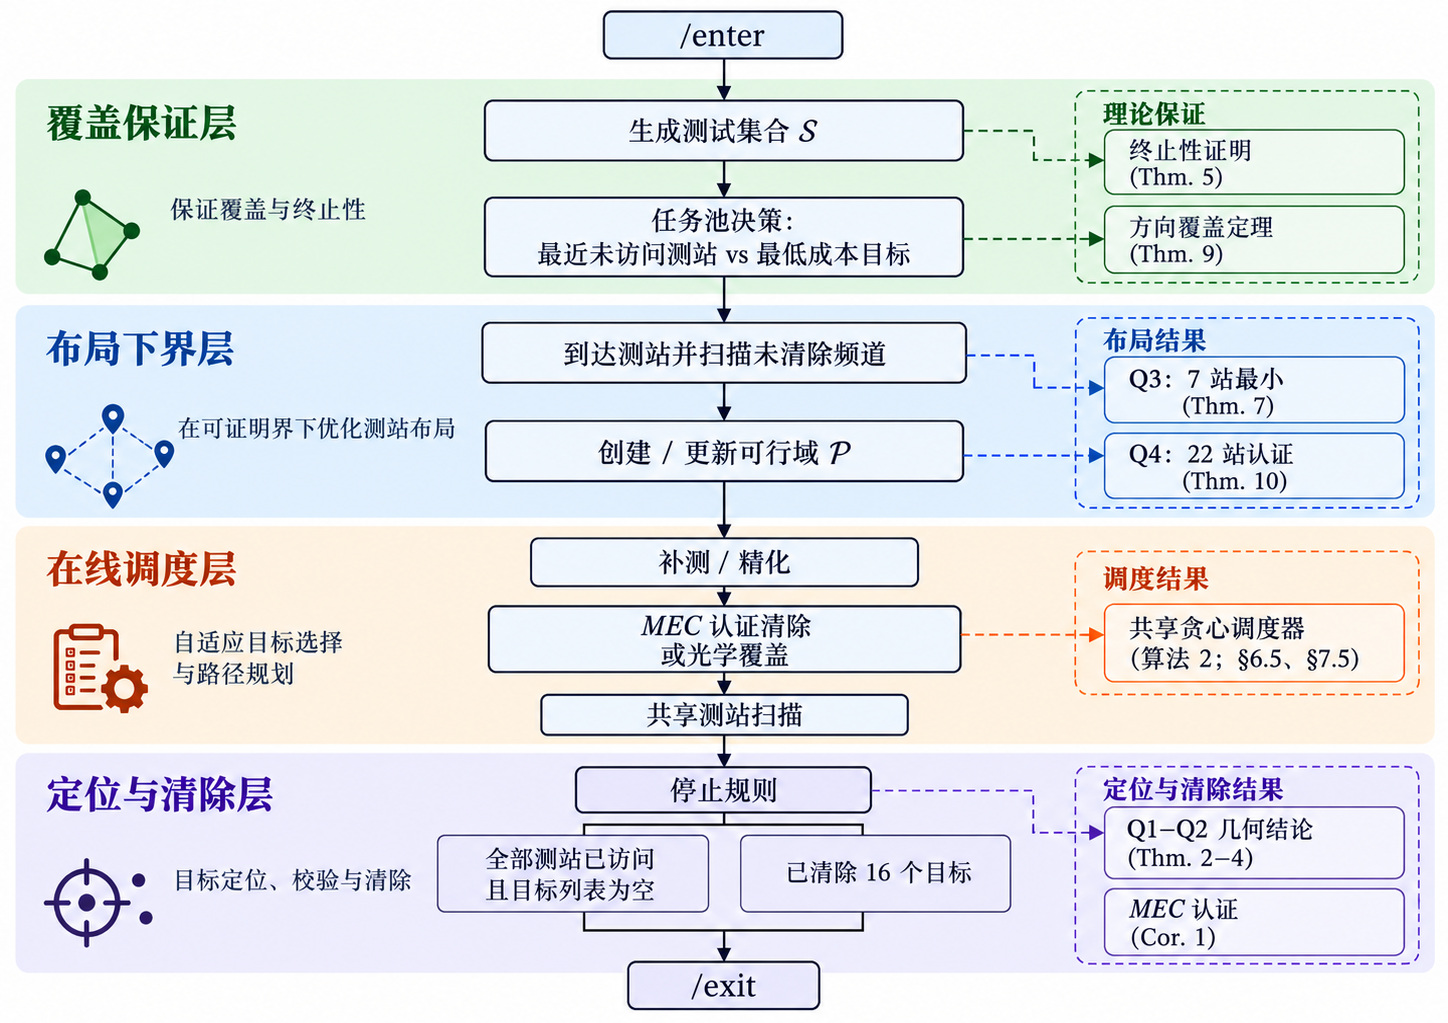
\includegraphics[width=\textwidth]{figures/fig-framework.png}
  \caption{总体求解框架：覆盖保证、布局下界、在线调度与定位清除四层}\label{fig:framework}
\end{figure}

\begin{table}[!htbp]
  \caption{数学保证、代码实现与逐例验收的对应}\label{tab:proof-impl}\centering\small
  \begin{tabularx}{\textwidth}{@{}L L L@{}}
    \toprule[1.5pt]
    数学保证 & 代码实现 & 逐例验收 \\
    \midrule[1pt]
    终止性（\cref{thm:term3}） & 走遍所有覆盖测站后才允许退出 & 逐例核对清除数 $=$ 真实源数 \\
    方向覆盖（\cref{thm:hull}） & 运行时 $20\mmet$ 粗网格凸包检查 & $h=1\mmet$ 网格证书 $1018.68$ 万点全部通过 \\
    认证清除（\cref{cor:certify}） & 仅当 $\mecr\le r_c-10^{-6}$ 才在圆心清除 & 清除点到真源距离 $\le20\mmet$ \\
    包含性不变量（\cref{eq:invariant}） & 目标圆外切、圆盘排除取凸包外近似 & 每时刻可行域与包围圆均含真源 \\
    \bottomrule[1.5pt]
  \end{tabularx}
\end{table}

\begin{table}[!htbp]
  \caption{在线决策流程的判定与动作}\label{tab:decision}\centering\small
  \begin{tabularx}{\textwidth}{@{}l L L@{}}
    \toprule[1.5pt]
    状态 & 判断条件 & 后续动作 \\
    \midrule[1pt]
    首测成功 & 返回 \texttt{direction} & 由方位约束建立可行域，进入定位 \\
    首测无信号 & 全向源返回 \texttt{no\_signal} & 以圆盘排除该站邻域；定向源改用其他测站 \\
    观测不足 & 可行域无界或仅 $1$ 条方位 & 走到第二测点或补测一次 \\
    可行域过大 & $\mecr>r_c$ & 圆心补测精化，仍不足则光学覆盖 \\
    认证通过 & $\mecr\le r_c-10^{-6}$ & 在最小包围圆圆心执行 \texttt{/clear} \\
    清除失败 & 接口拒绝或超时 & 限次重试，否则安全退出并留档 \\
    \bottomrule[1.5pt]
  \end{tabularx}
\end{table}

\subsection{四问的核心难点}

四问各自的核心困难可概括为：问题一要在有界角度误差下严格表示定位区域，并给出只依赖可行域的清除判据；问题二要让第二测点既保证收到信号又改善交会角，并说清两次测向的能力边界；问题三要在不知道源数与位置时证明“已全部发现”，并在保证全清下压缩固定成本；问题四中定向源使“距离覆盖”失效，需要新的方向覆盖条件。四问与四层的对应是：问题一提供定位证书（第\ref{sec:q1}节），问题二给出第二测点选择（第\ref{sec:q2}节），问题三完成全向源的覆盖与路径（第\ref{sec:q3}节），问题四给出定向源的方向覆盖与搜索布局（第\ref{sec:q4}节）。

\subsection{四个问题之间的关系}

需要强调，第三、四问是部分可观测的在线搜索控制问题：在走完所有测站之前，算法不知道还有几个源、在哪里，因此必须先回答“未发现源可能存在于哪些区域”和“何时可以安全结束”，才能借鉴路径优化的思想。

\paragraph{核心贡献.} 全文的主要贡献可凝练为四点：\textbf{其一}，建立“发现—定位—清除”的全覆盖保证框架，把终止条件建立在连续域几何覆盖上；\textbf{其二}，证明七站布局达到距离覆盖的理论下界（$6$ 站不可能）；\textbf{其三}，用凸包充要条件刻画定向源的方向覆盖，并给出 $22$ 站的连续域证书；\textbf{其四}，由时间构成诊断认定固定成本主导，据此把优化落到测站布局上。
\section{问题一：交会定位区域的直径算法与覆盖性判定}\label{sec:q1}

\subsection{从示向度读数到线性约束}

设在检测点 $s_k$ 处测得某干扰源的示向度为 $\theta_k$，误差界为 $\varepsilon$。由\cref{asu:bounded}，真源 $g$ 相对 $s_k$ 的真实方位角落在 $[\theta_k-\varepsilon,\theta_k+\varepsilon]$ 内，因此 $g$ 位于以 $s_k$ 为顶点、张角 $2\varepsilon$ 的\textbf{前向楔形}
\begin{equation}\label{eq:wedge}
  W_k=\Bigl\{x\in\R^2 \;\Bigm|\; \bigl[\uvec{\theta_k-\varepsilon},\,x-s_k\bigr]\ge 0,\quad
                                  \bigl[\uvec{\theta_k+\varepsilon},\,x-s_k\bigr]\le 0\Bigr\}
\end{equation}
之中，其中 $[\bm a,\bm b]=a_xb_y-a_yb_x$。定位区域即
\begin{equation}\label{eq:P}
  P=\bigcap_{k=1}^{K} W_k .
\end{equation}

\begin{lemma}[两条不等式已自动选出前向分支]\label{lem:forward}
当 $2\varepsilon<180^\circ$ 时，\cref{eq:wedge}恰好刻画以 $\uvec{\theta_k}$ 为轴、半角为 $\varepsilon$ 的单侧锥，而不包含背向方向。
\end{lemma}
\begin{proof}
令 $x-s_k=r\,\uvec{\varphi}$（$r>0$）。两条约束分别化为 $\sin(\varphi-\theta_k+\varepsilon)\ge0$ 与 $\sin(\varphi-\theta_k-\varepsilon)\le0$，即
$\varphi-\theta_k+\varepsilon\in[0,\pi]$ 且 $\varphi-\theta_k-\varepsilon\in[-\pi,0]\pmod{2\pi}$，两者之交为 $\varphi-\theta_k\in[-\varepsilon,\varepsilon]$。特别地取 $\varphi=\theta_k+180^\circ$ 时第一式给出 $-\sin\varepsilon<0$，故背向射线被排除。
\end{proof}

\cref{lem:forward}并非可有可无的细节：若把示向度处理成一条“带宽为 $2\varepsilon$ 的双向直线带”，则背向的一整块区域会被错误地保留，在多站交会时可能产生虚假的交集。

把\cref{eq:wedge}的两条约束写成行向量形式，$K$ 个检测点共给出 $m=2K$ 条线性不等式，于是
\begin{equation}\label{eq:poly}
  P=\{x\in\R^2 \;:\; \bm A x\le \bm b\},\qquad \bm A\in\R^{m\times2},\ \bm b\in\R^{m}.
\end{equation}
$P$ 是闭凸集，但\textbf{不一定有界}，也可能为空或退化。

\subsection{直径的计算：算法与正确性}

\begin{theorem}[直径在顶点上取到]\label{thm:diam}
设 $P$ 为有界闭凸多边形，顶点集为 $V(P)=\{v_1,\dots,v_k\}$，则
$\diam(P)=\max_{i<j}\|v_i-v_j\|$。
\end{theorem}
\begin{proof}
$\|\cdot\|$ 是凸函数，故对固定的 $y$，$x\mapsto\|x-y\|$ 在紧凸集 $P$ 上的最大值必在极点处取到；对 $y$ 再用一次同样的论证即可。由 Minkowski 定理，有界闭凸多边形的极点恰为其顶点。
\end{proof}

由\cref{thm:diam}，求直径只需枚举顶点对，而不必在边界上做连续优化。据此给出\cref{alg:diam}。它的关键不在于求直径这一步本身，而在于\textbf{先把四类情形分清楚，再计算}：直接对约束做顶点枚举而不判空、不判无界，会在读数互相矛盾或测站张角不足时输出毫无意义的数字。

\begin{algorithm}[!htbp]
\caption{有界误差交会定位区域的直径算法}\label{alg:diam}
\begin{algorithmic}[1]
\Require 检测点 $s_1,\dots,s_K$，示向度 $\theta_1,\dots,\theta_K$，误差界 $\varepsilon$
\Ensure 定位区域 $P$ 的状态（空／无界／有界）、顶点表与直径 $D$
\State 由\cref{eq:wedge}组装 $\bm A\in\R^{2K\times2}$，$\bm b\in\R^{2K}$
\State 解可行性线性规划 $\min\{0 \;:\; \bm Ax\le\bm b\}$
\If{不可行} \Return \textbf{空集}（读数与误差界相互矛盾，应报错而不是输出伪定位点）
\EndIf
\For{$\bm c\in\{(1,0),(-1,0),(0,1),(0,-1)\}$}
  \State 解 $\min\{\bm c^{\!\top}x \;:\; \bm Ax\le\bm b\}$
  \If{无下界} \Return \textbf{无界}，$D=+\infty$
  \EndIf
\EndFor
\State $V\gets\varnothing$
\For{每一对约束 $(i,j)$，$i<j$}
  \If{$\det(\bm a_i,\bm a_j)\ne0$}
    \State 解 $\bm a_i^{\!\top}x=b_i,\ \bm a_j^{\!\top}x=b_j$ 得交点 $x$
    \If{$\bm Ax\le\bm b+\tau\bm 1$ 且 $x\notin V$（按容差去重）} $V\gets V\cup\{x\}$
    \EndIf
  \EndIf
\EndFor
\State 以 $V$ 的重心为极点，按极角对 $V$ 排序，得到凸多边形顶点序列
\State $D\gets\max_{v_i,v_j\in V}\|v_i-v_j\|$ \Comment{线段与单点自然退化为 $D=\|v_1-v_2\|$ 与 $D=0$}
\State \Return \textbf{有界}，$V$，$D$
\end{algorithmic}
\end{algorithm}

\paragraph{五次线性规划各自的用途.} 需要说明的是，算法中的线性规划\emph{只用来判别 $P$ 的类型，不用来求顶点}。第 2 行的可行性规划取零目标，只问“约束组是否相容”；第 5 至 7 行的四次规划分别沿 $\pm x$、$\pm y$ 方向求极小，只要有一次报告目标无下界，$P$ 就在该方向上延伸至无穷，属于无界情形。四个坐标方向足以判定：二维多面体无界当且仅当其回收锥非平凡，而非平凡锥必与某个坐标半轴张成正夹角。判完类型之后，有界情形的顶点由第 9 至 14 行的“边界线两两求交、再逐个检验是否满足全部约束”得到，与线性规划无关。

\paragraph{复杂度.} 上述实现的开销为：$5$ 次二维线性规划（规模均为 $m$ 条约束、$2$ 个变量，可视为常数次）；顶点枚举 $O(m^2)$ 对交点，每个交点需 $O(m)$ 次可行性检验，合计 $O(m^3)$；最后直径枚举 $O(k^2)$。本题中单个源的检测点很少（$K\le4$，即 $m\le8$），这一实现完全够用，且代码短、边界情形容易查错。若检测点数很大，可换成半平面交（$O(m\log m)$）加旋转卡壳（$O(k)$）把总复杂度降到 $O(m\log m)$——这是一个\emph{替代实现}，本文提交的代码用的仍是前一种。

\paragraph{四类退化的处理.} $P$ 为空意味着读数与误差界不相容（例如误差界设小了），此时必须报错并排查角度约定、取整或坐标系，\emph{不能}静默地取一个近似交点；$P$ 无界出现在各楔形的方向锥未能互相封闭时（典型情形是只有一个检测点，或多个检测点近似共线且同侧），此时直径为 $+\infty$，用人为的大方框截断再报一个有限直径是错误的；$P$ 退化为线段或单点时，\cref{alg:diam}给出的 $D$ 自然正确，无需特判。

\subsection{以定位区域直径为直径的圆能否覆盖定位区域}

\begin{theorem}[覆盖性的充要条件与紧界]\label{thm:jung}
设 $P\subset\R^2$ 为有界闭凸集，$D=\diam(P)$，$\mecr=\mecr(P)$ 为最小包围圆半径。则
\begin{equation}\label{eq:jung}
  \frac{D}{2}\ \le\ \mecr\ \le\ \frac{D}{\sqrt3},
\end{equation}
右端为 Jung 不等式，两端均可取等。于是
\begin{itemize}
  \item 存在以 $D$ 为直径的圆覆盖 $P$，\textbf{当且仅当} $\mecr=D/2$；
  \item 一般情况下只能保证：以 $\dfrac{2D}{\sqrt3}\approx1.1547\,D$ 为直径的圆必能覆盖 $P$，且该系数不可改进。
\end{itemize}
\end{theorem}
\begin{proof}
左端：取 $p,q\in P$ 使 $\|p-q\|=D$，任何包含 $P$ 的圆都包含 $p,q$，故其半径不小于 $D/2$。右端即平面情形的 Jung 定理。取等：$P$ 为线段时 $\mecr=D/2$；$P$ 为边长 $D$ 的正三角形时 $\mecr=D/\sqrt3$。第一条由 $\mecr\ge D/2$ 立得。
\end{proof}

\paragraph{结论：一般不能覆盖.} 由\cref{thm:jung}，只要 $\mecr>D/2$，以 $D$ 为直径的圆无论圆心放在哪里都无法覆盖 $P$。这不是抽象反例，而是可以由真实的检测点与示向度产生的：

\begin{example}[三站交会给出 Jung 界上的正三角形]\label{exa:tri}
取三个检测点与读数
\[
  \begin{aligned}
  s_1&=(-1100,\,0), & \theta_1&=1^\circ;\\
  s_2&=(590,\,-952.6279), & \theta_2&=121^\circ;\\
  s_3&=(570,\,987.2690), & \theta_3&=241^\circ,
  \end{aligned}
\]
误差界 $\varepsilon=1^\circ$。按\cref{alg:diam}计算，$P$ 为有界三角形，顶点为
$(0,0)$、$(40,0)$、$(20,\,34.641016)$，即边长 $40\mmet$ 的正三角形。此时
\[
  D=40.000000\mmet,\qquad \mecr=23.094011\mmet,\qquad \frac{D}{2}=20\mmet,
\]
$\mecr/D=0.577350=1/\sqrt3$，恰好取到 Jung 不等式的等号。以 $D$ 为直径的圆（半径 $20\mmet$）\textbf{不能}覆盖该三角形，缺口为 $3.094011\mmet$，见\cref{fig:q1-counter}。
\end{example}

\begin{figure}[!htbp]
  \centering

  %% 画法建议：左子图画\cref{exa:tri}的三个检测点（远处，可用折断坐标轴或局部放大框）及三条示向度中心线与各自 $\pm1^\circ$ 的虚线，
  %% 交出的正三角形用浅色填充；右子图放大该三角形，叠加两个圆：半径 $D/2=20\mmet$ 的圆（红色虚线，可见三角形三个角伸出圆外）
  %% 与最小包围圆 $\mecr=23.094\mmet$（蓝色实线，恰好过三个顶点）。标注 $D=40\mmet$ 的一条边与 $\mecr/D=1/\sqrt3$。
  \fbox{\parbox[c][2.2cm][c]{0.86\textwidth}{\centering\small
  【待插图】（绘图要求见本段 \TeX{} 源码注释）}}
  \caption{以定位区域直径为直径的圆一般不能覆盖定位区域}\label{fig:q1-counter}
\end{figure}

\paragraph{什么时候可以覆盖：两站交会的情形.} 题目附图所示的\emph{两站}交会四边形，在两站到源的距离远大于区域尺度时趋于平行四边形；对这一类区域，同直径圆总是够用的。

\begin{lemma}[平行四边形的最小包围圆]\label{lem:para}
设 $P$ 为平行四边形，顶点为 $p,\ p+\bm u,\ p+\bm u+\bm v,\ p+\bm v$，则 $\mecr(P)=\diam(P)/2$，即以其直径为直径的圆一定能覆盖 $P$。
\end{lemma}
\begin{proof}
不妨设 $\bm u^{\!\top}\bm v\ge0$（否则把 $\bm v$ 换成 $-\bm v$ 并平移顶点标号，图形不变）。两条对角线的长度为 $\|\bm u\pm\bm v\|$，而
\[
  \|\bm u+\bm v\|^2-\|\bm u-\bm v\|^2=4\,\bm u^{\!\top}\bm v\ \ge 0,
\]
故 $\bm u+\bm v$ 是较长的对角线；又 $\|\bm u+\bm v\|^2=\|\bm u\|^2+\|\bm v\|^2+2\bm u^{\!\top}\bm v\ge\max(\|\bm u\|^2,\|\bm v\|^2)$，说明它也不短于任何一条边，于是 $\diam(P)=\|\bm u+\bm v\|$。

取圆心 $c=p+(\bm u+\bm v)/2$、半径 $\|\bm u+\bm v\|/2$。该圆过 $p$ 与 $p+\bm u+\bm v$；对另外两个顶点，
\[
  \bigl\|(p+\bm u)-c\bigr\|=\bigl\|(p+\bm v)-c\bigr\|=\frac{\|\bm u-\bm v\|}{2}\ \le\ \frac{\|\bm u+\bm v\|}{2},
\]
故四个顶点全在圆内或圆上，凸性给出 $P$ 被该圆覆盖，即 $\mecr(P)\le\diam(P)/2$。结合\cref{thm:jung}的左端不等式即得等号。
\end{proof}

\cref{lem:para}的论证只用到向量内积的符号，不需要对交会角作任何限制——这一点很重要，因为\cref{tab:q1-example}的第一个算例交会角为 $97.13^\circ$，已经是钝角。\cref{tab:q1-example}中 $\mecr$ 与 $D/2$ 在四位小数下完全相同，与引理一致。

\begin{table}[!htbp]
  \caption{两站交会的数值算例（真源 $g=(600,400)$，$\varepsilon=1^\circ$，读数含 $+0.6^\circ$ 与 $-0.4^\circ$ 的偏差）}
  \label{tab:q1-example}\centering\small
  \begin{tabular}{cccccccc}
    \toprule[1.5pt]
    $s_1$ & $s_2$ & 交会角 $\psi$ & 顶点数 & $D/\mmet$ & $\mecr/\mmet$ & $D/2$ & 可否一次认证清除 \\
    \midrule[1pt]
    $(0,0)$ & $(800,0)$  & $97.13^\circ$ & $4$ & $32.0756$ & $16.0378$ & $16.0378$ & 可（$\mecr\le20$） \\
    $(0,0)$ & $(1400,0)$ & $60.26^\circ$ & $4$ & $55.7265$ & $27.8632$ & $27.8632$ & 否，需光学兜底 \\
    \bottomrule[1.5pt]
  \end{tabular}
\end{table}

\noindent 两例中真源均满足全部线性约束，即 $g\in P$，符合\cref{asu:bounded}下的包含性要求。

\subsection{本问结论对后两问的决定性影响}

\cref{thm:jung}直接给出了后两问中\textbf{“何时可以一次性把源清掉”}的正确判据。由于清除成功的条件是清除点与源的距离不超过 $r_c=20\mmet$，而算法只知道 $g\in P$，故：

\begin{corollary}[认证清除判据]\label{cor:certify}
在 $c_*(P)$ 处执行一次 \texttt{/clear} 必定成功，当且仅当 $\mecr(P)\le r_c=20\mmet$。若仅已知直径，则
\begin{equation}\label{eq:diamsuff}
  D\le \sqrt3\,r_c=20\sqrt3\approx34.641\mmet
\end{equation}
是 $\mecr(P)\le r_c$ 的充分条件，且由\cref{exa:tri}该系数不可放宽到 $2r_c=40\mmet$。
\end{corollary}

因此，工程上常见的“定位区域直径小于 $2\times20=40\mmet$ 就能一次清除”的说法是\textbf{错误}的：\cref{exa:tri}中 $D=40\mmet$ 却存在距圆心 $23.09\mmet$ 的可能位置。本文后续算法一律以 $\mecr(P)\le20\mmet-10^{-6}$ 作为认证条件（保留浮点余量），而不使用直径判据；只有在需要一个只依赖直径的快速筛选时，才使用\cref{eq:diamsuff}。

\section{问题二：第二检测点的选择策略与候选区域}\label{sec:q2}

\subsection{问题的形式化与两个必须同时满足的要求}

设首个检测点为 $s_1$，测得某\emph{全向}源的示向度为 $\theta_1$。建立以 $s_1$ 为原点、$\uvec{\theta_1}$ 为 $x$ 轴正向、$\uvec{\theta_1+90^\circ}$ 为 $y$ 轴正向的局部坐标系。记真源在局部坐标下为
\begin{equation}\label{eq:localg}
  g=r\bigl(\cos\delta,\ \sin\delta\bigr),\qquad |\delta|\le\varepsilon,\quad 0\le r\le\rho\le\rho_{\max}=1500\mmet ,
\end{equation}
其中 $r$ 与该源的真实接收半径 $\rho$ 都\textbf{未知}，只知道 $\rho\ge\rho_{\min}=1000\mmet$，且因首站收到了信号必有 $r\le\rho$。第二检测点记为 $q=(a,b)$，其在原坐标下为 $q=s_1+a\,\uvec{\theta_1}+b\,\uvec{\theta_1+90^\circ}$。

一个“好”的第二检测点必须同时满足两个要求：

\begin{description}
  \item[要求 A（可用性）.] 在 $q$ 处必须\emph{确实能收到}该源的信号，否则这次移动与检测不能提供任何新的方位约束。由于 $r$ 与 $\rho$ 未知，这必须是一个\textbf{不依赖未知量的充分条件}。
  \item[要求 B（有效性）.] 两条视线的交会必须足够“横”，使得定位区域 $P=W_1\cap W_2$ 足够小。
\end{description}

二者与\textbf{移动代价} $\|q\|/v$ 构成三方权衡。下面分别给出要求 A 的精确刻画（\cref{thm:csafe}）与要求 B 的定量刻画（\cref{lem:psi}、\cref{eq:Rapprox}），再由二者导出选点策略。

\subsection{要求 A：保证接收的候选区域}

\begin{theorem}[保证接收的候选区域]\label{thm:csafe}
若第二检测点 $q=(a,b)$ 满足
\begin{equation}\label{eq:csafe}
  \mathcal C_{\rm safe}:\quad
  \begin{cases}
    a^2+b^2\le \rho_{\min}^2, \\[2pt]
    a^2+b^2\le 2\rho_{\min}\bigl(a\cos\varepsilon-|b|\sin\varepsilon\bigr),
  \end{cases}
\end{equation}
则\emph{无论真实源距 $r$ 与真实接收半径 $\rho$ 取何值}，在 $q$ 处一定能收到该全向源的信号。等价地，
\begin{equation}\label{eq:lens}
  \mathcal C_{\rm safe}
  = B\bigl(\bm 0,\rho_{\min}\bigr)\ \cap\
    B\bigl(\rho_{\min}\uvec{\varepsilon},\rho_{\min}\bigr)\ \cap\
    B\bigl(\rho_{\min}\uvec{-\varepsilon},\rho_{\min}\bigr),
\end{equation}
即三个半径为 $\rho_{\min}$ 的圆盘之交。
\end{theorem}

\begin{proof}
需要证明 $\|q-g\|\le\rho$。因 $\rho\ge\max(\rho_{\min},r)$，只需证 $\|q-g\|\le\max(\rho_{\min},r)$。

\emph{情形一：$r\le\rho_{\min}$.} 此时只需 $\|q-g\|\le\rho_{\min}$。函数 $h(r)=\|q-r\uvec{\delta}\|^2=r^2-2r\,q^{\!\top}\uvec{\delta}+\|q\|^2$ 关于 $r$ 是凸二次函数，故在区间 $[0,\rho_{\min}]$ 上的最大值必在端点取到。$r=0$ 时 $h=\|q\|^2\le\rho_{\min}^2$，即\cref{eq:csafe}第一式；$r=\rho_{\min}$ 时要求 $\|q-\rho_{\min}\uvec{\delta}\|\le\rho_{\min}$，展开即 $\|q\|^2\le2\rho_{\min}q^{\!\top}\uvec{\delta}$。由于 $|\delta|\le\varepsilon$，
$q^{\!\top}\uvec{\delta}=a\cos\delta+b\sin\delta\ge a\cos\varepsilon-|b|\sin\varepsilon$，于是\cref{eq:csafe}第二式是对所有允许的 $\delta$ 成立的充分条件。

\emph{情形二：$r>\rho_{\min}$.} 此时 $\rho\ge r$，只需 $\|q-g\|\le r$，即 $\|q\|^2\le 2r\,q^{\!\top}\uvec{\delta}$。由第二式可知 $q^{\!\top}\uvec{\delta}>0$，故右端关于 $r$ 单调增，最紧的情形是 $r=\rho_{\min}$，回到第二式。

最后，$\|q\|^2\le2\rho_{\min}q^{\!\top}\uvec{\pm\varepsilon}$ 等价于 $\|q-\rho_{\min}\uvec{\pm\varepsilon}\|\le\rho_{\min}$，而第二式恰为 $\delta=+\varepsilon$ 与 $\delta=-\varepsilon$ 两种情形同时成立，故得\cref{eq:lens}。
\end{proof}

\begin{corollary}[候选区域的极值点]\label{cor:extreme}
$\mathcal C_{\rm safe}$ 中横向偏移的最大值为
\begin{equation}\label{eq:bmax}
  |b|_{\max}=\rho_{\min}\sin(60^\circ-\varepsilon)=1000\sin59^\circ=857.167\mmet ,
\end{equation}
在 $a=\rho_{\min}\cos(60^\circ-\varepsilon)=515.038\mmet$ 处取到；前向偏移的最大值为 $a_{\max}=\rho_{\min}=1000\mmet$（此时 $b=0$）。
\end{corollary}
\begin{proof}
$B(\bm 0,\rho_{\min})$ 与 $B(\rho_{\min}\uvec{-\varepsilon},\rho_{\min})$ 是两个半径相等、圆心相距 $\rho_{\min}$ 的圆盘，其边界交点位于 $\rho_{\min}\uvec{-\varepsilon\pm60^\circ}$，上方交点即 $\rho_{\min}\uvec{60^\circ-\varepsilon}$，代入即得。
\end{proof}

\begin{figure}[!htbp]
  \centering

  %% 画法建议：在局部坐标系中画三个半径 $1000\mmet$ 的圆（圆心分别在原点、$1000\uvec{1^\circ}$、$1000\uvec{-1^\circ}$），
  %% 其公共部分填色即 $\mathcal C_{\rm safe}$；标出极值点 $(515.0,\pm857.2)$ 与 $(1000,0)$；
  %% 叠加首测楔形（$\pm1^\circ$ 的窄扇形）；再用等值线叠加“$r_1=1500$ 时的 $\mecr$ 一阶估计”，
  %% 可直观看到 $\mecr$ 随 $|b|$ 增大而下降、随移动距离增大而代价上升；
  %% 最后标出本文实际采用的 $(200,100)$ 与历史基线 $(650,250)$ 两个点。
  \fbox{\parbox[c][2.2cm][c]{0.86\textwidth}{\centering\small
  【待插图】（绘图要求见本段 \TeX{} 源码注释）}}
  \caption{保证接收的第二检测点候选区域及其等代价线}\label{fig:q2-region}
\end{figure}

\cref{fig:q2-region}给出了 $\mathcal C_{\rm safe}$ 的形状及其与定位精度、移动代价的关系。

\paragraph{关于候选区域的三点说明.} 其一，$\mathcal C_{\rm safe}$ 是\emph{充分}条件而非充要条件：实际可用的点可能更多（例如源距很近时），但那需要用到未知的 $r$ 与 $\rho$，不能作为策略依据。其二，$\mathcal C_{\rm safe}$ 允许 $q$ 落在 $1800\mmet$ 目标圆之外，这是合法的——附件明确允许机器狗走出目标区域。其三，原点 $q=\bm 0$ 虽然平凡地满足\cref{eq:csafe}，却必须排除：在同一地点重复检测得到的是同一读数（\cref{asu:bounded}），不提供任何新约束，而下文的交会角与点线距离公式在该点也同时退化为零。实现中要求
\begin{equation}\label{eq:qnonzero}
  \|q-s_1\|\ \ge\ q_{\min}=100\mmet ,
\end{equation}
这一门槛同时被共享测站的“与已有采样点至少相距 $100\mmet$”规则复用（见\cref{tab:shared}）。

\subsection{要求 B：交会角与定位区域尺度}

\begin{lemma}[交会角由横向偏移单独决定]\label{lem:psi}
设 $\psi$ 为两条视线在真源 $g$ 处的夹角，$L$ 为过 $s_1$ 与 $g$ 的直线，则
\begin{equation}\label{eq:sinpsi}
  \sin\psi=\frac{\dist(q,L)}{\|q-g\|},\qquad
  \dist(q,L)=\bigl|b\cos\delta-a\sin\delta\bigr|\ \ge\ |b|\cos\varepsilon-a\sin\varepsilon .
\end{equation}
\end{lemma}
\begin{proof}
在三角形 $s_1gq$ 中，$g$ 处的内角为 $\psi$（或其补角，正弦相同）。由正弦定理
$\|q-s_1\|/\sin\psi=\|q-g\|/\sin\angle(s_1)$，而 $\dist(q,L)=\|q-s_1\|\sin\angle(s_1)$，整理即得。第二式由 $L$ 与局部 $x$ 轴夹角为 $\delta$、$|\delta|\le\varepsilon$ 直接算出。
\end{proof}

\cref{lem:psi}给出了本问最重要的结构性结论：\textbf{交会角的下界只由横向偏移 $|b|$（相对于第二段视距 $r_2=\|q-g\|$）决定，与前进距离 $a$ 无关}。“沿着示向度方向一直往前走”对改善交会角毫无帮助，只能缩短 $r_2$。

在 $\bar\varepsilon$ 为小角的一阶近似下，两条楔形在 $g$ 附近可视为宽度
$w_1=2r_1\tan\bar\varepsilon$、$w_2=2r_2\tan\bar\varepsilon$ 的直条带（$r_1=\|g-s_1\|$，$r_2=\|g-q\|$），其交为平行四边形。由\cref{lem:para}，该平行四边形的最小包围圆半径恰为长对角线之半：
\begin{equation}\label{eq:Rapprox}
  \mecr\ \approx\ \frac{1}{2}\cdot\frac{\sqrt{w_1^2+w_2^2+2w_1w_2|\cos\psi|}}{\sin\psi},
  \qquad \sin\psi=\frac{\dist(q,L)}{r_2}.
\end{equation}
把 $w_i$ 代入并用 $\sqrt{w_1^2+w_2^2+2w_1w_2|\cos\psi|}\le w_1+w_2$ 放大，可得一个便于讨论趋势的上界
\begin{equation}\label{eq:Rbound}
  \mecr\ \lesssim\ \frac{(r_1+r_2)\,r_2\tan\bar\varepsilon}{\dist(q,L)} .
\end{equation}
它清楚地显示：$\mecr$ 大致正比于 $r_1r_2$、反比于横向偏移。

\paragraph{一阶估计的适用范围.} \cref{eq:Rapprox}把楔形当成等宽条带，忽略了“楔形宽度沿距离线性增长”这一事实，因此只在 $r_2$ 相对区域尺度足够大、且交会角不过分尖锐时才准确。把它与\cref{tab:q2-enum}的精确枚举对照可以看到：横向偏移较大（$b\ge450\mmet$）时两者相差约 $15\%$，而 $b=100\mmet$ 的极尖锐交会下一阶估计会高估近一倍。\textbf{因此本文只用\cref{eq:Rapprox}解释趋势与做量级判断，所有作为结论依据的数值一律取自精确枚举或严格构造。}

\subsection{两次测向不足以保证认证清除}

一个自然的想法是：既然第二次测向能把区域缩小，那么再挑得讲究一些，是不是就能把 $\mecr$ 压进 $20\mmet$，从而省掉光学覆盖？答案是否定的，而且这一点可以\emph{严格}地证明——不依赖任何近似公式。

\begin{theorem}[两次测向的分辨极限]\label{thm:twobearing}
存在两个相距 $41\mmet$ 的源位置，使得无论第二检测点取在 $\mathcal C_{\rm safe}$ 中的哪一点，都存在一组容许的测向误差，令两个源产生\emph{完全相同}的两次观测。由于 $41\mmet>2r_c=40\mmet$，不存在任何一点能同时位于两源的 $20\mmet$ 清除范围内。因此，仅凭两次测向无法保证一次认证清除。
\end{theorem}

\begin{proof}
取首检测点 $s_1$ 为原点，并考虑两个候选源
\[
  g_1=(1500,\,0),\qquad g_2=(1459,\,0),\qquad \|g_1-g_2\|=41\mmet ,
\]
二者的接收半径都取 $\rho_{\max}=1500\mmet$。它们相对 $s_1$ 的真实方位角都是 $0^\circ$，故首次读数 $\theta_1=0^\circ$ 对两者同时相容（误差取零即可）。

设第二检测点为 $q\in\mathcal C_{\rm safe}\subseteq B(\bm 0,\rho_{\min})$，即 $\|q\|\le1000\mmet$。记 $\alpha(q)=\angle\,g_1qg_2$ 为两源在 $q$ 处的张角。由于 $g_1,g_2$ 都在 $x$ 轴上，直接计算给出：在圆周 $\|q\|=\rho_q$ 上 $\alpha$ 的最大值为
\begin{equation}\label{eq:resolve}
  \alpha_{\max}(\rho_q)=\arctan\frac{\|g_1-g_2\|\cdot\rho_q}
       {\sqrt{\bigl(\|g_1\|^2-\rho_q^2\bigr)\bigl(\|g_2\|^2-\rho_q^2\bigr)}},
\end{equation}
且 $\alpha_{\max}$ 关于 $\rho_q$ 单调增，故在整个圆盘 $\|q\|\le1000$ 上的上确界在边界取到。代入数值，
\[
  \alpha_{\max}(1000)=\arctan\frac{41\times1000}{\sqrt{(1500^2-1000^2)(1459^2-1000^2)}}
  =1.976940^\circ\ <\ 2\varepsilon=2^\circ .
\]
于是对任意 $q$，取第二次读数 $\theta_2$ 为两条真实方位角的中点，则两个假设各自所需的误差都不超过 $\alpha_{\max}/2=0.988^\circ\le\varepsilon$，均为容许误差。又因 $\|q-g_i\|\le\|q\|+\|g_i\|$ 且实际计算给出两段视距均不超过 $700\mmet<\rho_{\max}$，两个源在 $q$ 处都确实可被接收。

因此 $g_1$ 与 $g_2$ 产生同一组观测 $\{(s_1,\theta_1),(q,\theta_2)\}$，任何只依赖观测的算法都无法区分二者。若某个清除点 $x$ 能保证成功，则必须同时有 $\|x-g_1\|\le20$ 与 $\|x-g_2\|\le20$，从而 $\|g_1-g_2\|\le40<41$，矛盾。
\end{proof}

\cref{eq:resolve}还顺带给出了一个有用的刻画：\textbf{两次测向能分辨的最小间距随源距急剧变差}。在 $\rho_q=1000\mmet$ 下，$r_1=1100,1200,1300,1400,1500\mmet$ 对应的不可分辨间距分别为 $7.1,\ 14.7,\ 23.0,\ 31.9,\ 41.5\mmet$；它恰在 $r_1\approx1485\mmet$ 处越过 $2r_c=40\mmet$。也就是说，\emph{只有最远的那一小段距离上才会出现“两次测向原理上不够用”的情形}，而题目给定的接收半径上界正好是 $1500\mmet$，这一段无法回避。

按\cref{eq:Rapprox}在 $\mathcal C_{\rm safe}$ 上做一阶全域搜索，也得到一致的结论：$r_1=1500\mmet$ 时可达到的最小 $\mecr$ 约为 $61\mmet$（取 $q\approx(816,578)$，此处 $\|q\|=1000\mmet$，光走过去就要 $200\msec$）。这个数字是一阶估计，量级上与\cref{thm:twobearing}的严格结论相符。

这一结论有三个直接后果，贯穿第三、四问。\textbf{其一，光学覆盖兜底不可省略}：任何“先两次测向、再一次清除”的流水线都不完备，必须保留一个对整个可行域的、有连续覆盖证明的清除点列。\textbf{其二，不宜盲目追求正交交会}：远距离源反正要进入光学覆盖，为把 $\mecr$ 从数百米降到几十米而多走 $800\mmet$（$160\msec$）往往并不划算。\textbf{其三，近源应优先获得第二次测向}：由\cref{eq:Rbound}，$\mecr$ 大致正比于 $r_1r_2$，对近源而言两次测向常常已经够用——以 $(200,100)$ 为第二点时，首测距离在 $380\mmet$ 以内的源基本可一次认证清除（\cref{tab:q2-need}）。

\begin{table}[!htbp]
  \caption{不同候选第二点的定位效果与移动代价（$\mecr$ 为按\cref{eq:Rapprox}算出的一阶估计，$\bar\varepsilon=1.005^\circ$，单位 m）}\label{tab:q2-need}\centering\small
  \begin{tabular}{ccccccc}
    \toprule[1.5pt]
    候选点 $(a,b)$ & 移动/m & 移动/s & $r_1=500$ & $r_1=1000$ & $r_1=1500$ & 可认证的最大 $r_1$ \\
    \midrule[1pt]
    $(200,100)$ & $223.6$ & $44.7$ & $44.7$ & $255.0$ & $640.8$ & $377\mmet$ \\
    $(250,100)$ & $269.3$ & $53.9$ & $35.7$ & $232.7$ & $605.3$ & $416\mmet$ \\
    $(300,300)$ & $424.3$ & $84.9$ & $16.1$ & $76.9$  & $196.5$ & $556\mmet$ \\
    $(500,250)$ & $559.0$ & $111.8$& $9.8$  & $59.7$  & $181.7$ & --- \\
    $(650,250)$ & $696.4$ & $139.3$& $14.2$ & $41.4$  & $146.9$ & --- \\
    $(750,450)$ & $874.6$ & $174.9$& $17.6$ & $26.7$  & $78.2$  & --- \\
    $(515,857)^{\dagger}$ & $999.8$ & $200.0$& $17.5$ & $34.6$  & $70.3$ & --- \\
    \bottomrule[1.5pt]
  \end{tabular}\\[2pt]
  \footnotesize $\dagger$ 为\cref{cor:extreme}给出的最大横向偏移点；所有候选点均在 $\mathcal C_{\rm safe}$ 内。
  末列为使一阶 $\mecr$ 降到 $20\mmet$ 以内的最大首测距离；后四个点的 $\mecr$ 随 $r_1$ 非单调（源可能落在第二点附近），无单一阈值，故不填。
\end{table}

\subsection{精确枚举验证与选点策略}

为避免只依赖一阶近似，本文对 $12$ 个候选点做了精确枚举：源距取 $21$ 个值、首测偏差取 $3$ 个方向、第二测偏差取 $3$ 个方向，共 $189$ 个组合，逐一按\cref{alg:diam}计算精确的交会多边形与其直径，取样本内最坏值，结果见\cref{tab:q2-enum}。

\begin{table}[!htbp]
  \caption{$12$ 个候选第二点的精确枚举结果（每点 $189$ 个组合，$\varepsilon=1^\circ$）}\label{tab:q2-enum}\centering\small
  \begin{tabular}{@{}cccc@{\hspace{2.2em}}cccc@{}}
    \toprule[1.5pt]
    前进 $a$/m & 侧移 $b$/m & 移动/s & 最坏直径/m & 前进 $a$/m & 侧移 $b$/m & 移动/s & 最坏直径/m \\
    \midrule[1pt]
    $250$ & $100$ & $53.85$  & $631.03$ & $650$ & $100$ & $131.53$ & $414.19$ \\
    $250$ & $250$ & $70.71$  & $361.97$ & $650$ & $250$ & $139.28$ & $230.30$ \\
    $250$ & $450$ & $102.96$ & $240.56$ & $650$ & $450$ & $158.11$ & $156.35$ \\
    $500$ & $100$ & $101.98$ & $494.05$ & $750$ & $100$ & $151.33$ & $362.11$ \\
    $500$ & $250$ & $111.80$ & $277.46$ & $750$ & $250$ & $158.11$ & $200.52$ \\
    $500$ & $450$ & $134.54$ & $185.97$ & $750$ & $450$ & $174.93$ & $138.06$ \\
    \bottomrule[1.5pt]
  \end{tabular}
\end{table}

数据印证了\cref{lem:psi}：\textbf{固定 $a$ 时，最坏直径随 $b$ 增大而迅速下降（侧移由 $250$ 加到 $450\mmet$ 可使直径减半）；而固定 $b$ 时，增大 $a$ 的收益明显更小}。同时，$12$ 个候选中表现最好的 $(750,450)$ 最坏直径仍有 $138.06\mmet$，对应 $\mecr\approx69.0\mmet$，远大于 $r_c=20\mmet$——这与\cref{thm:twobearing}的严格结论互相印证。

\paragraph{数字口径的统一说明.} 本节出现了三类数，量纲与来源都不同：\cref{tab:q2-need}是\textbf{一阶估计的半径}，\cref{tab:q2-enum}是\textbf{精确枚举的直径}（除以二才与前者可比），\cref{thm:twobearing}的 $41\mmet$ 则是\textbf{两个不可分辨源的间距}。三者在“两次测向不足以认证清除”这一点上结论一致，但只有\cref{thm:twobearing}是严格的，其余两者仅作量级参照。

\paragraph{选点策略.} 综上，第二检测点的选择应当按下列顺序：
\begin{enumerate}
  \item \textbf{可行性优先}：$q\in\mathcal C_{\rm safe}$（\cref{eq:csafe}），保证一定收得到信号；
  \item \textbf{左右镜像取近}：$b$ 取正负两个镜像位置中综合代价更小的一侧；
  \item \textbf{以“完成任务所需时间”而非“区域面积”为目标}：最小化
  \begin{equation}\label{eq:q2cost}
    J(q)=\underbrace{\frac{\|q-p_{\rm cur}\|}{v}}_{\text{走到第二点}}
        +\underbrace{t_m+t_s}_{\text{检测与切频}}
        +\underbrace{\widehat{C}_{\rm clear}\bigl(P(q)\bigr)}_{\text{此后清除该源的估计代价}},
  \end{equation}
  其中 $\widehat C_{\rm clear}$ 为“若 $\mecr\le r_c$ 则走到圆心清除，否则按光学覆盖点列走一遍”的保守估计。
\end{enumerate}

\paragraph{单目标最优不等于整局最优.} 本文在第三、四问中实际采用的是较短的 $(a,b)=(200,\pm100)$，而不是\cref{tab:q2-enum}中单目标意义下更优的 $(750,450)$。原因有三：其一，由\cref{thm:twobearing}，远距离源无论如何都要走光学覆盖，把 $\mecr$ 从几百米降到几十米换来的扫描节省，抵不过多走 $650\mmet$（$130\msec$）的代价；其二，多目标场景中\emph{同一次移动可以为多个频道提供观测}（共享测站，见\cref{sec:q3:shared}），第二测点不再需要为单个目标“专程”远行；其三，走远之后机器狗离主巡站路线更远，会带来后续折返。

本文用固定种子的配对实验验证了这一判断：在 $\{100,150,200,250,300\}\times\{50,100,150,200\}$ 的离散集合上按信息增益与移动代价\emph{自适应}选点，与固定 $(200,100)$ 相比，第三问 $263.920\to265.518\msec/$源、第四问 $505.344\to508.205\msec/$源，两问均值与最坏值均无改善（清除率均为 $100\%$）。因此正式方案保留固定的 $(200,\pm100)$，并把“要不要再测一次”的判断交给\cref{sec:q3:refine}的补测精化与\cref{sec:q4:online}的扫描成本门控。

\section{问题三：全向干扰源的自动搜索、定位与清除}\label{sec:q3}

\subsection{三层结构与终止证明}

第三问的难点不在“怎样清除一个已知的源”，而在“怎样证明已经没有源了”。本文把策略分成\textbf{发现—定位—清除}三层，其中发现层承担终止证明的责任。

\begin{definition}[距离覆盖测站集]\label{def:cover3}
称测站集 $\mathcal S$ 对目标区域 $\Dreg$ 具有\emph{距离覆盖}，若
\begin{equation}\label{eq:cover3}
  d_{\max}(\mathcal S):=\max_{x\in\Dreg}\ \min_{s\in\mathcal S}\ \|x-s\|\ \le\ \rho_{\min}=1000\mmet .
\end{equation}
\end{definition}

\begin{theorem}[终止的正确性]\label{thm:term3}
设 $\mathcal S$ 具有距离覆盖。若算法在每个 $s\in\mathcal S$ 处都对每个尚未成功清除的频道检测过一次，并清除了由此发现的所有目标，则 $\Dreg$ 内不存在未被清除的全向干扰源。
\end{theorem}
\begin{proof}
反设频道 $c$ 上还存在未清除源 $g\in\Dreg$。由\cref{eq:cover3}存在 $s\in\mathcal S$ 使 $\|s-g\|\le1000\le\rho$。全向源覆盖角为 $360^\circ$，故在 $s$ 处检测频道 $c$ 必定返回 \texttt{direction} 或 \texttt{near}，于是 $g$ 会被发现并进入目标列表，与“所有发现的目标均已清除”矛盾。
\end{proof}

\cref{thm:term3}说明：合法的停止理由只有两个——\textbf{(i)} 覆盖测站全部访问完毕且目标列表清空；\textbf{(ii)} 已成功清除 $16$ 个源，达到题设数量上界。“连续若干次没有收到信号”“已经清了 $10$ 个”“$20$ 个频道各扫过一遍”都\emph{不是}有效的终止证明。

\subsection{发现层：七站布局及其最优性}\label{sec:q3:layout}

\subsubsection{最坏覆盖距离的解析式}

由\cref{sec:analysis:fixed}，固定成本与测站数成正比，因此应在\cref{eq:cover3}的约束下尽量减少站数、缩短巡回。本文采用“圆心 $+$ 半径 $r$ 的正六边形”共 $7$ 站的布局
\begin{equation}\label{eq:hex}
  \mathcal S_7=\{\bm 0\}\cup\bigl\{r\,\uvec{60^\circ k}\ :\ k=0,1,\dots,5\bigr\}.
\end{equation}

\begin{theorem}[七站布局的最坏覆盖距离]\label{thm:hexcover}
对 $0<r\le\sqrt3R$，
\begin{equation}\label{eq:dmax}
  d_{\max}(\mathcal S_7)=\max\left\{\frac{r}{\sqrt3},\ \sqrt{R^2+r^2-\sqrt3\,Rr}\right\}.
\end{equation}
\end{theorem}
\begin{proof}
设 $x\in\Dreg$，$t=\|x\|$。六个环点均匀分布，故存在一个环点 $s_k$ 使 $x$ 与 $s_k$ 的极角差 $\phi$ 满足 $|\phi|\le30^\circ$，于是
$\|x-s_k\|=\sqrt{t^2+r^2-2tr\cos\phi}\le\sqrt{t^2+r^2-\sqrt3\,tr}=:g(t)$。
又圆心站给出距离 $t$，故最近站距离不超过 $f(t)=\min\{t,g(t)\}$。

比较两支：$t\le g(t)\iff t^2\le t^2+r^2-\sqrt3tr\iff t\le r/\sqrt3$。因此
$f(t)=t$ 于 $[0,r/\sqrt3]$，$f(t)=g(t)$ 于 $[r/\sqrt3,R]$。前段最大值为 $r/\sqrt3$。后段 $g$ 是关于 $t$ 的二次根式，$g'(t)\propto2t-\sqrt3r$，在 $t=\sqrt3r/2$ 取极小，故在闭区间 $[r/\sqrt3,R]$ 上的最大值在端点取到，为 $\max\{g(r/\sqrt3),g(R)\}=\max\{r/\sqrt3,\ \sqrt{R^2+r^2-\sqrt3Rr}\}$。合并即得\cref{eq:dmax}。上界可达：$x$ 取 $t=r/\sqrt3$ 且极角恰在两环点之间（Voronoi 三重点），或 $x$ 取目标圆边界上两环点角平分方向的点。
\end{proof}

\begin{corollary}[环半径的可行区间与最优值]\label{cor:ring}
取 $R=1800\mmet$、$\rho_{\min}=1000\mmet$，$d_{\max}\le\rho_{\min}$ 当且仅当
\begin{equation}\label{eq:ringrange}
  \begin{aligned}
  &r\in\bigl[\,r_-,\ r_+\,\bigr],\\
  &r_-=\frac{\sqrt3R-\sqrt{3R^2-4(R^2-\rho_{\min}^2)}}{2}=1122.956\mmet,\\
  &r_+=\sqrt3\,\rho_{\min}=1732.051\mmet .
  \end{aligned}
\end{equation}
$d_{\max}(r)$ 在 $r^\star=\dfrac{\sqrt3}{2}R=1558.846\mmet$ 处取最小值 $R/2=900\mmet$。
\end{corollary}

\paragraph{为什么不取覆盖最优的 $r^\star$.} 覆盖只是\emph{约束}而非\emph{目标}。$r$ 越小，六个环点越靠内，巡站路线越短，而且发现目标后的第二测点、补测点与清除点也都更靠近主路线。因此本文在可行区间内取靠近下界的 $r=1150\mmet$，此时
\begin{equation}
  d_{\max}=\sqrt{1800^2+1150^2-\sqrt3\times1800\times1150}=988.5114\mmet<1000\mmet,
\end{equation}
覆盖余量 $11.4886\mmet$。$5\mmet$ 网格加边界采样的数值核对（$61445$ 个位置）与该解析值一致。程序在启动时用\cref{eq:dmax}重新校验，不满足覆盖条件即\emph{拒绝运行}，避免误改参数导致保证失效。

\cref{fig:q3-layout}给出了该布局的覆盖示意与 $d_{\max}(r)$ 曲线。实验上，$r$ 取 $1250,1300,\dots,1450$ 的扫描全部慢于 $1150$；而 $r<1122.956$ 会直接破坏覆盖保证。也就是说，\textbf{$r=1150\mmet$ 已经贴着可行下界}，这一维参数上不再有可挖掘的空间。

\subsubsection{七站是保证发现的最小站数}

\begin{theorem}[站数下界]\label{thm:seven}
在 $R=1800\mmet$、$\rho_{\min}=1000\mmet$ 的条件下，任何具有距离覆盖的测站集至少包含 $7$ 个站；\cref{eq:hex}取 $r\in[r_-,r_+]$ 时达到该下界。
\end{theorem}
\begin{proof}
\cref{eq:cover3}等价于用 $|\mathcal S|$ 个半径 $\rho_{\min}$ 的闭圆盘覆盖半径 $R$ 的圆盘，即覆盖半径比为 $R/\rho_{\min}=1.8$。Bezdek 证明了 $6$ 个单位圆盘所能覆盖的圆的最大半径为
$1.7988\ldots<1.8$\cite{bezdek,bezdek2,kershner}，故 $|\mathcal S|\le6$ 不可能；而 $\mathcal S_7$ 在 $r\in[r_-,r_+]$ 时满足覆盖，故 $7$ 可达。
\end{proof}

为了从反面确认这一结论的紧性（并检验“少一站能省多少”），本文另外实现了一个\emph{不保证覆盖}的六站实验入口，结果见\cref{tab:q3six}。

\begin{table}[!htbp]
  \caption{六站布局实验（独立入口，默认方案未采用）}\label{tab:q3six}\centering\small
  \begin{tabularx}{\textwidth}{@{}L c c c c c@{}}
    \toprule[1.5pt]
    布局 & 最坏未覆盖距离/m & 单源漏检概率 & $120$ 例均值 s/源 & 与 $7$ 站配对差 & 更快局数 \\
    \midrule[1pt]
    $7$ 站（默认） & $988.5$（有保证） & $0$ & $258.6$ & --- & --- \\
    $6$ 站环 $960\mmet$   & $1102.0$ & $\approx4\times10^{-4}$ & $256.1$ & $-2.5$ & $69/120$（漏 $1$ 源） \\
    $6$ 站环 $1000\mmet$  & $1062.9$ & $\approx2\times10^{-4}$ & $257.2$ & $-1.4$ & $61/120$（无漏） \\
    $6$ 站环 $1040\mmet$  & $1043.5$ & $\approx8\times10^{-5}$ & $257.9$ & $-0.7$ & $63/120$（无漏） \\
    \bottomrule[1.5pt]
  \end{tabularx}
\end{table}

用 Nelder--Mead 做过六站极小极大优化，最坏未覆盖距离最低只能压到约 $1003\mmet$（接近理论值 $1000.7\mmet$），仍然超过 $1000\mmet$。更重要的是：\textbf{去掉一个站只节省约 $6\msec/$源的扫描，却因为失去圆心站而使首次发现更远、清除路程更长，移动增加约 $4\msec/$源，净收益仅 $1\sim2\msec/$源，代价是引入约万分之二的单源漏检概率}。在“清除率是硬约束”的准则下这一交换不可接受，因此正式方案坚持七站。这表明\textbf{第三问的发现层已接近其几何下界}。

\begin{figure}[!htbp]
  \centering
  \fbox{\parbox[c][6.5cm][c]{0.9\textwidth}{\centering\textbf{【此处插图】图~\thefigure：第三问七站布局与覆盖验证}\\[4pt]
  \small 画法建议：左子图画 $R=1800\mmet$ 目标圆、$7$ 个测站（圆心 $+$ 环半径 $1150\mmet$ 的六点）与它们的 Voronoi 剖分，
  每站叠加半径 $1000\mmet$ 的接收圆（半透明），可见并集完整覆盖目标圆；标出两个最坏点（$r/\sqrt3=663.95\mmet$ 的 Voronoi 三重点
  与边界上 $988.51\mmet$ 的点）。右子图画 $d_{\max}(r)$ 随环半径 $r$ 的变化曲线（\cref{eq:dmax}），
  横轴 $r\in[900,1800]$，标出可行区间 $[1122.96,1732.05]$、最优点 $r^\star=1558.85$、以及实际取值 $r=1150$ 及其余量 $11.49\mmet$。}}
  \caption{七站布局的覆盖证明与环半径的可行区间}\label{fig:q3-layout}
\end{figure}

\subsection{定位层：有界误差可行域}\label{sec:q3:loc}

对每个已发现频道 $c$ 维护一个凸可行域 $P_c$，其不变量是
\begin{equation}\label{eq:invariant}
  \textbf{（包含性不变量）}\qquad g_c\in P_c\ \text{恒成立}.
\end{equation}

\paragraph{（i）初始化.} 首次收到 \texttt{direction} 时，以检测点 $p$ 为顶点构造包含真实扇区的三角形外包
\begin{equation}
  P_c^{(0)}=\conv\bigl\{p,\ p+\rho_{\max}\uvec{\theta}-w\bm n,\ p+\rho_{\max}\uvec{\theta}+w\bm n\bigr\},
  \quad w=\rho_{\max}\tan\bar\varepsilon,\ \bm n\perp\uvec{\theta}.
\end{equation}
它外包了半径 $\rho_{\max}$、半角 $\bar\varepsilon$ 的扇形，因此无需猜测源距。

\paragraph{（ii）新方位裁剪.} 每获得一条新的有效示向度，按\cref{eq:wedge}生成两条半平面并求交：$P_c\leftarrow P_c\cap W$。若结果为空，说明模型假设与观测矛盾，程序\emph{报错并保留日志}，而不是取一个近似点继续。

\paragraph{（iii）目标圆外包约束.} 所有源都在 $\Dreg$ 内，故可以再交上目标圆。为保持多边形表示，本文用 $48$ 条\textbf{支撑半平面}
$\bm n_j^{\!\top}x\le R+10^{-7}$（$\bm n_j$ 均匀取 $48$ 个方向）作为圆的\emph{外切}近似。这里必须是外切而不是内接：内接多边形会把靠近圆边界的一圈真实位置切掉，可能使边界源脱离 $P_c$，破坏\cref{eq:invariant}。

\paragraph{（iv）无信号的距离排除（仅第三问）.} 这是第三问相对第四问独有的信息优势。

\begin{theorem}[无信号排除]\label{thm:nosignal}
第三问中所有源都是全向源。若在点 $s$ 检测频道 $c$ 返回 \texttt{no\_signal}，而频道 $c$ 上仍存在未清除的源 $g_c$，则
$\|s-g_c\|>\rho_c\ge\rho_{\min}$，即 $g_c\notin B(s,\rho_{\min})$。
\end{theorem}

于是可令 $P_c\leftarrow \conv\bigl(P_c\setminus B^\circ(s,\rho_{\min})\bigr)$。注意 $P_c\setminus B^\circ$ 一般\emph{非凸}，本文取其凸包作为\textbf{保守外近似}：这可能重新包含一小部分已被排除的区域（约束变松），但绝不会误删真源。实现中排除半径取 $\rho_{\min}-10^{-4}$，为浮点计算留余量。

\paragraph{一次必须记录的失败.} 在圆盘排除约束的首轮验证中，曾有一例的几何证书失效：该局虽然最终清除了全部源，程序内部却报出“可行域排除了真源”。根因是：重复施加圆盘排除时，一个理论上位于边界的交点被浮点判为落在圆盘\emph{内部}，相应二次方程的根又略微超出线段参数范围，导致边界顶点被错误丢弃，多次裁剪后可行域出现了\emph{不保守}的收缩。修复措施为：用平方距离容差保留边界顶点、对接近端点的根做范围容许与夹取、点数不足或凸包退化时保留输入多边形，并增加重复约束的回归测试。该案例的种子、报错与修复前后对比见附录~\ref{app:debug}。

这次失败给出一条重要教训，也是本文的一个方法论主张：\textbf{“结果全部清除”不能替代对中间几何不变量的检查}。所有实验都必须逐条核验可行多边形与包围圆是否真的包含真源。\cref{fig:q3-shrink}展示了可行域在上述四类约束下逐步收缩直至可以认证清除的完整过程。

\begin{figure}[!htbp]
  \centering
  \fbox{\parbox[c][6.5cm][c]{0.9\textwidth}{\centering\textbf{【此处插图】图~\thefigure：可行域的逐步收缩与认证清除}\\[4pt]
  \small 画法建议：四联子图，同一坐标范围。(a) 首次测向后的三角形外包 $P^{(0)}$（细长扇形外包，长 $1500\mmet$）；
  (b) 第二次测向后 $P^{(0)}\cap W_2$（细长四边形），标出最小包围圆及其半径；
  (c) 叠加一次 \texttt{no\_signal} 的圆盘排除（画出 $B(s,1000)$ 的弧与取凸包后的保守外近似，用两种填充区分“精确差集”与“凸包外近似”，
  说明外近似只会变松、不会误删真源）；(d) 圆心补测后 $\mecr\le20\mmet$，画出认证清除圆与真源位置。
  每个子图标注 $\mecr$ 的数值，并始终把真源标成一个醒目的点以显示包含性不变量始终成立。}}
  \caption{有界误差可行域的收缩过程}\label{fig:q3-shrink}
\end{figure}

\subsection{清除层：认证清除、光学兜底与补测精化}\label{sec:q3:refine}

\paragraph{（i）认证清除.} 由\cref{cor:certify}，当 $\mecr(P_c)\le r_c-10^{-6}$ 时，在最小包围圆圆心 $c_*(P_c)$ 处执行一次 \texttt{/clear} 必定成功。最小包围圆按“$1$、$2$ 或 $3$ 个支撑顶点”穷举候选圆心并逐一校验，凸多边形只需检查顶点。

\paragraph{（ii）光学覆盖兜底.} 若 $\mecr>r_c$，用边长 $h_{\rm opt}=25\mmet$ 的方格覆盖 $P_c$，保留所有与 $P_c$ 相交的格，在各格中心依次尝试清除。覆盖正确性来自
\begin{equation}\label{eq:grid}
  \frac{h_{\rm opt}}{\sqrt2}=\frac{25}{\sqrt2}=17.677670\mmet<20\mmet=r_c,
\end{equation}
即格内任意点到格心的距离都在清除半径内；由于真源必在 $P_c$ 内、$P_c$ 被这些格覆盖，故必有一格成功。遍历采用按列蛇形路径，并根据当前位置选择从哪一端进入。

\paragraph{（iii）补测精化.} 认证清除与光学兜底之间存在一个过渡区间：$\mecr$ 只比 $20\mmet$ 略大（例如 $60\mmet$），却可能需要在上百米的网格上逐点尝试清除。为此加入圆心补测：当 $r_c<\mecr\le300\mmet$ 时，\textbf{先走到 $c_*(P_c)$ 再测一次}——该移动与后续清除路径高度重合，因此边际成本较低；若仍 $>20\mmet$，则沿新方位的垂线方向横移 $60\mmet$ 再补测一次；此后才进入光学网格。$100$ 例留出验证：平均 $262.6\to260.0\msec/$源，\textbf{每源失败清除次数由 $3.00$ 次降到 $0.38$ 次}，$64$ 例更快、$36$ 例更慢、最大单例退步 $30.9\msec/$源。

\subsection{调度层：搜索与目标处理的混合贪心}\label{sec:q3:shared}

早期版本采用“到一个站 $\to$ 扫完 $\to$ 处理本站发现的全部目标 $\to$ 再去下一站”的分批流程，会产生大量折返。当前版本把\textbf{搜索任务}与\textbf{目标任务}放进同一个任务池，每一步比较：

\begin{itemize}
  \item 去最近未访问测站的代价：$\|s^*-p_{\rm cur}\|$；
  \item 处理待清除目标 $c$ 的代价：
  \begin{equation}\label{eq:q3cost}
    J(c)=
    \begin{cases}
      \|q_c-p_{\rm cur}\|+\|q_c-c_*(P_c)\|, & \text{还需补一条方位},\\[2pt]
      \|x_c-p_{\rm cur}\|, & \text{已可直接处理},
    \end{cases}
  \end{equation}
\end{itemize}
其中 $q_c$ 为第二测点，$x_c$ 为 \texttt{near} 点或最小包围圆圆心 $c_*(P_c)$；取二者中较小者执行。这样机器狗可以“顺路”经过新的测站，也可以在靠近时提前把近处目标处理掉。目标状态\emph{跨测站保留}，不再每到一站就清空。

\paragraph{共享测站（shared scan）.} 一次移动应当尽量服务多个目标。到达第二测点或完成一次清除后，算法检查其他待处理频道：若当前位置对该频道\emph{确有观测价值}，就顺便补测一次。筛选条件见\cref{tab:shared}，其作用是防止共享测量无限增加——它们是\emph{选择动作的启发式}，不提供额外的接收保证，也不参与任何正确性论证。

\begin{table}[!htbp]
  \caption{共享测站的筛选条件}\label{tab:shared}\centering
  \begin{tabular}{lc}
    \toprule[1.5pt]
    条件 & 阈值 \\
    \midrule[1pt]
    与该目标已有采样点的最小距离 & $\ge100\mmet$ \\
    目标估计中心到当前位置的距离 & $\le1300\mmet$ \\
    估计交会角的正弦 & $\ge0.12$ \\
    每个目标的额外共享检测次数 & $\le4$ \\
    已有有效方位数 & $<3$ 时才继续 \\
    已清除或已获得 \texttt{near} 的目标 & 跳过 \\
    \bottomrule[1.5pt]
  \end{tabular}
\end{table}

\subsection{算法总览}

把上述四层合在一起，得到\cref{alg:q3}。

\begin{algorithm}[!htbp]
\caption{第三问：七站覆盖 $+$ 混合贪心的在线搜索、定位与清除}\label{alg:q3}
\begin{algorithmic}[1]
\Require 目标圆半径 $R$，接收半径下界 $\rho_{\min}$，误差界 $\bar\varepsilon$，环半径 $r=1150\mmet$
\Ensure 全部干扰源被清除
\State 调用 \texttt{/enter}；$p_{\rm cur}\gets(0,0)$，当前频道 $\gets1$，$\mathcal C_{\rm done}\gets\varnothing$，轨迹表 $\mathcal Q\gets\varnothing$
\State 由\cref{eq:hex}生成 $\mathcal S_7$ 并用\cref{eq:dmax}校验覆盖；不满足则拒绝运行
\While{$\mathcal S_7\ne\varnothing$ 或 $\mathcal Q$ 中仍有未清除频道}
  \State $c^\star\gets\arg\min_{c\in\mathcal Q\setminus\mathcal C_{\rm done}}J(c)$ \Comment{\cref{eq:q3cost}}
  \State $s^\star\gets\arg\min_{s\in\mathcal S_7}\|s-p_{\rm cur}\|$
  \If{$\|s^\star-p_{\rm cur}\|<J(c^\star)$} \Comment{搜索更划算}
    \State 走到 $s^\star$ 并从 $\mathcal S_7$ 移除；对每个未清除频道 $c$ 依次检测（当前频道优先，其余升序）
    \State 若 $c\in\mathcal Q$ 则更新 $P_c$，否则在收到信号时新建轨迹并施加\cref{thm:nosignal}与目标圆约束
  \Else \Comment{处理目标更划算}
    \If{$c^\star$ 尚需补一条方位}
      \State 走到第二测点 $q_{c^\star}=\text{origin}+200\,\uvec{\theta}\pm100\,\bm n$（取综合代价小的一侧）并检测，更新 $P_{c^\star}$
      \State 共享测站扫描（排除 $c^\star$）
    \EndIf
    \State 圆心补测精化（\cref{sec:q3:refine}(iii)）
    \If{$\mecr(P_{c^\star})\le r_c-10^{-6}$} 在 $c_*(P_{c^\star})$ 处清除
    \Else\ 按 $25\mmet$ 方格蛇形遍历 $P_{c^\star}$ 逐格尝试清除
    \EndIf
    \State 共享测站扫描
  \EndIf
  \If{$|\mathcal C_{\rm done}|=16$} \textbf{break} \Comment{题设数量上界}
  \EndIf
\EndWhile
\State 调用 \texttt{/exit}
\end{algorithmic}
\end{algorithm}

\paragraph{虚拟时间上界.} 所有行动点都在以原点为心、$2000\mmet$ 为半径的圆内，任意两点距离不超过 $4000\mmet$。$7$ 个测站每站至多 $20$ 次含切频的检测（$120\msec$）；至多 $16$ 个目标，每个目标至多两段全局跳转、一条保守长度 $6500\mmet$ 的光学路线、若干次检测与至多 $183$ 次清除尝试。于是
\begin{equation}
  T\le 7\Bigl(\frac{4000}{5}+120\Bigr)+16\Bigl[\frac{2\times4000+6500}{5}+6\times6+183\times3+5\Bigr]
  \approx6.2\times10^{4}\msec\ \ll\ 3.6\times10^{5}\msec,
\end{equation}
远小于虚拟时间上限，也说明算法不可能因死循环而被强制终止。实际演练中整局虚拟时间约 $3300\msec$，现实程序运行时间 $1.7\sim2.4\msec$，相对 $1200\msec$ 的限制有三个数量级的余量。

\subsection{实验结果与消融}

\cref{fig:q3-track}给出一局完整任务的行走轨迹，可直观看到巡站与目标处理如何交错进行。所有本地实验均使用与开发阶段\emph{不重叠}的新种子做留出验证，并逐例核验：清除数等于真实源数、每次成功清除的实际距离 $\le20\mmet$、可行多边形与包围圆均包含真源、逐动作时间与\cref{eq:objective}一致。

\begin{table}[!htbp]
  \caption{第三问历次结构性改进的配对实验（单位：虚拟秒/源，两版均 $100\%$ 清除）}\label{tab:q3paired}\centering
  \begin{tabular}{lcccc}
    \toprule[1.5pt]
    改进 & 数据集 & 对照 & 候选 & 下降 \\
    \midrule[1pt]
    单次测向 $\to$ 两次测向 & $40$ 例，$498$ 源 & $977.71$ & $764.71$ & $21.79\%$ \\
    动态处理顺序 $+$ 共享测站 & $100$ 例，$1310$ 源 & $723.82$ & $653.11$ & $9.77\%$ \\
    $25$ 站网格 $\to$ $7$ 站解析覆盖 & $100$ 例，$1308$ 源 & $654.53$ & $346.62$ & $47.04\%$ \\
    环半径 $1150$ $+$ 混合贪心调度 & $100$ 例，$1315$ 源 & $343.73$ & $263.86$ & $23.24\%$ \\
    （同上，压力集） & $70$ 例，$890$ 源 & $336.31$ & $281.83$ & $16.20\%$ \\
    圆心补测精化 & $100$ 例留出 & $262.6$ & $260.0$ & $1.0\%$ \\
    \bottomrule[1.5pt]
  \end{tabular}\\[2pt]
  \footnotesize 各行使用的案例集合不同，\textbf{不能把各行降幅连乘}得到一个“总提升”。
\end{table}

\begin{figure}[!htbp]
  \centering
  \fbox{\parbox[c][6.5cm][c]{0.9\textwidth}{\centering\textbf{【此处插图】图~\thefigure：第三问一局完整轨迹}\\[4pt]
  \small 画法建议：取一局具有代表性的演练（例如 $n=14$、$\bar T=266.6\msec/$源），画出 $1800\mmet$ 目标圆、$7$ 个测站、
  机器狗的完整行走轨迹（按时间用渐变色，起点 $(0,0)$ 标出），每个源的真实位置用叉号、成功清除点用圆圈，
  失败的光学尝试点用小灰点；右上角小图给出累计虚拟时间随动作序号的阶梯曲线，并按动作类型着色。
  另可并排放一张对照图：$25$ 站旧版本在同一案例上的轨迹，直观展示路程差异。}}
  \caption{第三问典型局的行走轨迹与时间累积}\label{fig:q3-track}
\end{figure}

\cref{tab:q3paired}中收益最大的一行是测站布局（$47.04\%$），这与\cref{sec:analysis:fixed}的固定成本分析相吻合。特别地，混合贪心一行的成本分解显示：候选版平均\emph{少走} $5946\mmet$（约 $1189\msec$），代价是平均\emph{多做} $17.3$ 次检测与 $18.3$ 次失败清除（约 $141\msec$）。这正体现了\cref{sec:q1}以来的一贯取舍——\textbf{用少量额外测量换取大量移动节省}，而不是机械地减少动作次数。

\begin{table}[!htbp]
  \caption{第三问被否决的改进方案（均完成完整配对实验，清除率均为 $100\%$）}\label{tab:q3reject}\centering
  \begin{tabularx}{\textwidth}{>{\raggedright\arraybackslash}p{4.4cm} c c L}
    \toprule[1.5pt]
    方案 & 对照 s/源 & 候选 s/源 & 否决原因 \\
    \midrule[1pt]
    两步前瞻调度 $J(a)=C(p,a)+\lambda\min_bC(a,b)$ & $263.920$ & $292.795$ & 总移动 $12583\to14452\mmet$，$\mathrm{P}_{95}$ 亦恶化；复杂度上升而性能下降 \\
    非凸可行域（保留 \texttt{no\_signal} 挖洞后的非凸单元） & $263.920$ & $264.943$ & 单元碎片化，平均光学格数 $100.1\to102.3$，区域缩小未转化为更短路径 \\
    自适应第二测点（$5\times4$ 离散集合） & $263.920$ & $265.518$ & 均值与最坏值均恶化，见\cref{sec:q2} \\
    主动搜索（按未知区域覆盖收益选站） & $251.70$ & $260.95$ & 提前减少搜索后已发现目标测向不足，光学成本上升 \\
    \bottomrule[1.5pt]
  \end{tabularx}
\end{table}

\subsection{理论下界与优化空间}\label{sec:q3:lb}

为判断“还能优化多少”，本文建立一个下界模型：任何满足覆盖保证的策略都至少要
\textbf{(i)} 走遍 $7$ 个测站（下界取该站集的最短哈密顿路，目标处理段用随机点巡回的渐近公式 $0.7124\sqrt{NA}$ 估计不可避免的额外行程）；
\textbf{(ii)} 在所有站上排除空频道（未占用频道数 $\times$ 站数 $\times6\msec$，已发现频道平均扫半数站）；
\textbf{(iii)} 对每个源至少一次第二测点往返与一次成功清除。结果见\cref{tab:q3lb}。

\begin{table}[!htbp]
  \caption{第三问的时间下界与现有方案的差距（单位：虚拟秒）}\label{tab:q3lb}\centering
  \begin{tabular}{cccccccc}
    \toprule[1.5pt]
    源数 $n$ & 路线下界 & 扫描下界 & 每源附加 & 总下界 & 下界 s/源 & 现有本地 s/源 & 差距 \\
    \midrule[1pt]
    $10$ & $1874$ & $750$ & $310$ & $2934$ & $293$ & $310$ & $6\%$ \\
    $13$ & $2030$ & $700$ & $403$ & $3133$ & $241$ & $265$ & $9\%$ \\
    $16$ & $2180$ & $696$ & $496$ & $3372$ & $211$ & $226$ & $7\%$ \\
    \bottomrule[1.5pt]
  \end{tabular}
\end{table}

现有方案距下界只有 $6\%\sim9\%$，剩余差距来自巡站与目标处理交错的调度损失以及最坏情形余量。结合\cref{thm:seven}（站数不能再减）与\cref{cor:ring}（环半径已贴下界），本文认为\textbf{第三问的优化重点已从“搜索覆盖”转向“定位精度与光学覆盖开销”}，继续堆叠更复杂的调度器不再是有效方向。

\section{问题四：混合全向源与定向源的检测与清除}\label{sec:q4}

\subsection{第三问的覆盖条件为什么不能照搬}

第四问中每个源可能是定向源，其有效覆盖范围是以定向方向 $d$ 为轴、张角 $180^\circ$ 的闭半平面。于是“可见”的判据从单纯的距离变成距离与方向的合取：
\begin{equation}\label{eq:visible}
  \text{测站 } s \text{ 能发现位于 } g\text{、朝向 } d \text{ 的源}
  \iff \|s-g\|\le\rho\ \ \text{且}\ \ d^{\!\top}(s-g)\ge0 .
\end{equation}

这带来两个本质变化。其一，“附近有一个站”不再足够：离源最近的那个站完全可能落在天线背面。其二，\texttt{no\_signal} 不再携带距离信息——在 $s$ 处收不到频道 $c$，可能是距离超限，也可能只是背向，因此\cref{thm:nosignal}的圆盘排除在第四问不再适用，必须在实现上严格隔离。这是两问算法最重要的一处不对称。为方便叙述，记
\begin{equation}\label{eq:Tset}
  \mathcal N_\rho(g)=\bigl\{s\in\mathcal S\ \big|\ \|s-g\|\le\rho\bigr\} .
\end{equation}

\subsection{方向覆盖的充要条件}

\begin{theorem}：\textbf{凸包等价条件}．\label{thm:hull}
位于 $g$ 的源对任意未知朝向 $d$ 都存在可见测站，当且仅当
\begin{equation}\label{eq:hullcond}
  g\in\conv \mathcal N_\rho(g).
\end{equation}
\end{theorem}
\begin{proof}
（充分性）设 $g\in\conv \mathcal N_\rho(g)$，则存在 $s_1,\dots,s_k\in \mathcal N_\rho(g)$ 与 $\lambda_i\ge0$，$\sum\lambda_i=1$，使 $g=\sum\lambda_is_i$。于是对任意单位向量 $d$，
\[
  \sum_{i}\lambda_i\,d^{\!\top}(s_i-g)=d^{\!\top}\Bigl(\sum_i\lambda_is_i-g\Bigr)=0 .
\]
一组和为零的加权项不可能全部严格为负，故存在 $i$ 使 $d^{\!\top}(s_i-g)\ge0$；又 $\|s_i-g\|\le\rho$，由\cref{eq:visible}该站可见。

（必要性）设 $g\notin\conv \mathcal N_\rho(g)$。$\conv \mathcal N_\rho(g)$ 是紧凸集，由凸集分离定理存在单位向量 $d$ 与 $\alpha>0$ 使 $d^{\!\top}(s-g)\le-\alpha<0$ 对一切 $s\in \mathcal N_\rho(g)$ 成立。取该 $d$ 为定向方向，则所有距离足够近的站都落在天线背面，而距离超过 $\rho$ 的站本来就收不到，故无可见站。
\end{proof}

取 $\rho=\rho_{\min}=1000\mmet$，\cref{eq:hullcond}对区域内每一点成立即给出保证发现的\textbf{充要}条件。

\paragraph{与三角剖分条件的比较.} 早期版本（$49$ 站方格、$27$ 站三角网格、$25$ 站双环）用的是一个充分条件：把区域剖分成直径小于 $\rho_{\min}$ 的单元，源必落在某个单元内，而单元顶点既在接收范围内，又由凸组合关系保证至少一个位于前发射半平面。这要求相邻站之间的距离都小于 $\rho_{\min}$，站数因此下不去。\cref{thm:hull}放松了这一点：$\mathcal N_\rho(g)$ 中的站\textbf{不必两两相邻}，只要 $g$ 落在它们的凸包内即可。正是这一差别让测站数从 $25$ 减到 $22$——当前布局中内环 $(990,0)$ 与外环 $(1616,933)$ 相距 $1123.6\mmet>1000\mmet$，任何基于剖分的论证都覆盖不了它，而凸包条件依然成立。

\subsection{连续域的网格证书}\label{sec:q4:cert}

\cref{eq:hullcond}是对连续统中每一点的要求，不能靠有限采样“验证”。本文用一个带余量的网格证书把连续域问题化为有限检查。

\begin{theorem}：\textbf{网格证书}．\label{thm:cert}
取网格步长 $h$，令 $\delta=h/\sqrt2$。若对覆盖 $\Dreg$ 外扩 $\delta$ 的每一个网格点 $g$ 都有
\begin{equation}\label{eq:certcond}
  B(g,\delta)\ \subseteq\ \conv \mathcal N_{\rho-\delta}(g),
\end{equation}
则 $\Dreg$ 中任意一点 $p$ 都满足 $p\in\conv \mathcal N_{\rho}(p)$。
\end{theorem}
\begin{proof}
任取 $p\in\Dreg$，设 $g$ 为距 $p$ 最近的网格点，则 $\|p-g\|\le h/\sqrt2=\delta$。
其一，对任意 $s\in \mathcal N_{\rho-\delta}(g)$，有 $\|s-p\|\le\|s-g\|+\|g-p\|\le(\rho-\delta)+\delta=\rho$，故
$\mathcal N_{\rho-\delta}(g)\subseteq \mathcal N_\rho(p)$，从而 $\conv \mathcal N_{\rho-\delta}(g)\subseteq\conv \mathcal N_\rho(p)$。
其二，$p\in B(g,\delta)\subseteq\conv \mathcal N_{\rho-\delta}(g)$。二者合并即得 $p\in\conv \mathcal N_\rho(p)$。
\end{proof}

\cref{eq:certcond}中“包含一个半径 $\delta$ 的圆盘”这一要求等价于 $g$ 到凸包各支撑超平面的距离都不小于 $\delta$，即余量 $\mathrm{slack}(g)\ge\delta$，可由凸包的超平面表示直接算出（负值表示 $g$ 在凸包外）。

\paragraph{认证结果.} 布局搜索中考察过的全部候选（含各自的余量与是否通过证书）列于附录~\ref{app:sens}的\cref{tab:q4search}，最终采用的布局见\cref{tab:q4layout}与\cref{fig:q4-layout}。对该 $22$ 站布局取 $h=1\mmet$、$\delta=0.7071\mmet$，检查 $10\,186\,813$ 个网格点，全部通过，\textbf{最小余量为 $1.7331\mmet>\delta$}（最坏点位于 $(-1738,-471)$），计算耗时约 $12\msec$。运行时程序还会用 $20\mmet$ 粗网格再做一次凸包检查（余量 $2.417\mmet$），测站列表不满足覆盖时拒绝运行。

\subsection{$22$ 站布局：连续域证书与减站边界}\label{sec:q4:lower}

\subsubsection{连续域证书与结论范围}

\paragraph{结论的范围.} \textbf{可行性是严格的}——\cref{tab:q4layout}给出的具体布局通过\cref{thm:cert}意义下的连续域证书，对任意位置与朝向的源都保证发现；\textbf{不可行性则是受限的}——本文在“圆心 $+$ 正内环 $+$ 正外环”布局族内、配合局部搜索，找不到任何 $\le21$ 站的布局通过同一证书。需强调：这不排除某个不规则 $21$ 站布局仍可行，故 $22$ 是\textbf{本文找到并认证过的最小站数}（其最优性尚未证明）。

\subsubsection{减站边界与工程取舍}

\paragraph{减站的边界.} 三条引理说明减站会在三处碰壁：外环少于 $12$ 站时边界弧上出现凸包无法覆盖的点；去掉圆心站会使朝外源不可见；内环少于 $9$ 站时证书在 $(-100,100)$ 附近出现负余量。其中只有第一条是解析结论，后两条是特定布局上的数值验证（陈述与证明见附录~\ref{app:q4}）。

\begin{table}[!htbp]
  \caption{第四问采用的 $22$ 站认证布局}\label{tab:q4layout}\centering
  \begin{tabular}{lccc}
    \toprule[1.5pt]
    组成 & 站数 & 半径/m & 角度 \\
    \midrule[1pt]
    圆心站 & $1$  & $0$    & --- \\
    内环   & $9$  & $990$  & $0^\circ,40^\circ,\dots,320^\circ$ \\
    外环   & $12$ & $1866$ & $0^\circ,30^\circ,\dots,330^\circ$ \\
    \bottomrule[1.5pt]
  \end{tabular}\\[2pt]
  \footnotesize 最近邻巡回长度 $17940.2\mmet$（约 $3588\msec$）；相邻内环站间距 $677.1\mmet$；相邻外环站间距 $966.0\mmet$。
\end{table}

\paragraph{工程决策：$22$ 站与 $25$ 站的取舍.} 综合以上，本文以 $22$ 站为默认：它在题设参数下通过严格连续域证书，且巡站路径更短；$25$ 站解析布局作为保守备用保留。程序在启动时用 $20\mmet$ 粗网格复核，若当前参数下证书不满足（例如接收半径下界被调低到 $990\mmet$，$22$ 站约 $6\sim10\mmet$ 的余量消失），则拒绝使用 $22$ 站并回退到 $25$ 站。题目明确允许机器狗走出目标区域，故外环站与区域外第二测点都合规，且与 $2000000\mmet$ 的坐标上限相距甚远。

\begin{figure}[!htbp]
  \centering
  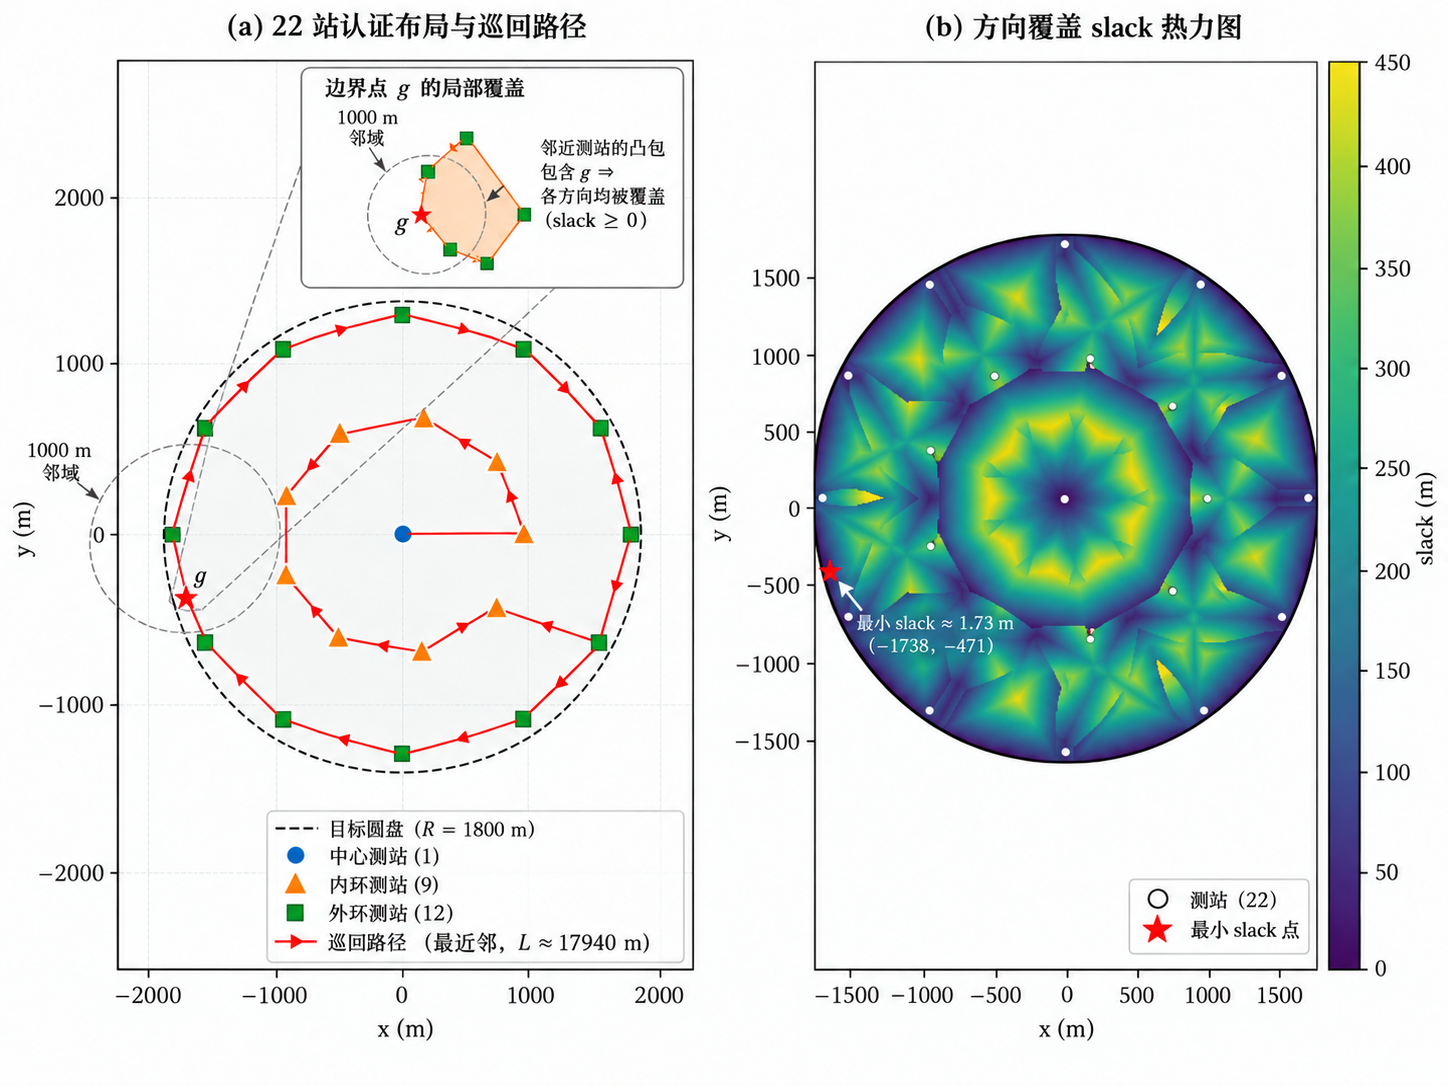
\includegraphics[width=\textwidth]{figures/fig-q4-layout.png}
  \caption{$22$ 站布局的方向覆盖证书}\label{fig:q4-layout}
\end{figure}

\subsection{在线层：选择性测量、有界等待与认证条带覆盖}\label{sec:q4:online}

第四问的定位层与第三问共用\cref{sec:q3:loc}的可行域递推与目标圆外包，但去掉\cref{thm:nosignal}的圆盘排除。在此基础上加入下列针对定向源的改进。

\paragraph{选择性重测.}

到达一个测站后，未发现的频道必须全部检测（这是终止证明的要求，不可省略）；但对已发现的频道，重复测量常常价值很低。设当前站为 $s$、目标可行域为 $P_c$，只有同时满足
\begin{equation}\label{eq:selective}
  \dist(s,P_c)\le950\mmet
  \quad\text{且}\quad
  \Bigl(\sin\widehat\psi\ge0.3\ \ \text{或}\ \ \min_{p\in\mathcal P_c}\|s-p\|\ge300\mmet\Bigr)
\end{equation}
时才重测，其中 $\widehat\psi$ 是以 $c_*(P_c)$ 为顶点、由已有采样点与 $s$ 张成的估计交会角，$\mathcal P_c$ 为已有采样点集。已经可以认证清除或已收到 \texttt{near} 的目标直接跳过。

\paragraph{有界等待与圆心补测.}

若某目标只有一条方位线，而后续巡站路线上正好有测站能提供第二条方位线（距可行域不超过 $950\mmet$），就可以推迟处理，等这次顺手可达的观测，省下一趟专程往返。为防止无限等待与错误等待，设了三重限制：只等一次；首次发现点距当前位置超过 $1400\mmet$ 时不等；在目标圆之外首次发现的目标不等——外环站能首次发现它，多半意味着该源朝外发射，后续站往往全部落在天线背面。

补测精化与第三问同理，只是阈值更紧：$\mecr\in(20,150]\mmet$ 时先走到 $c_*(P_c)$ 补测一次，若仍不够则沿新方位的垂线横移 $60\mmet$ 再补一次。

\paragraph{认证条带覆盖.}

$25\mmet$ 方格兜底（\cref{eq:grid}）只利用了清除圆的内接正方形，面积利用率为 $2/\pi\approx63.7\%$。本文改用沿首测方向的条带矩形覆盖：把 $P_c$ 沿 $\uvec{\theta}$ 切成宽 $w$ 的条，再在每条内沿横向切成高
\begin{equation}\label{eq:strip}
  h(w)=2\sqrt{r'^2-\left(\frac{w}{2}\right)^{2}},\qquad r'=r_c-0.1=19.9\mmet
\end{equation}
的矩形，取矩形中心为清除点。此时矩形四角到中心的距离恰为 $\sqrt{(w/2)^2+(h/2)^2}=r'<r_c$，由凸性整个矩形都落在清除圆内，覆盖性得证。$w$ 在 $\{1.25,1.5,1.7,1.9\}\times r'$ 中取；例如 $w=1.5r'=29.85\mmet$ 时 $h=26.32\mmet$，单点覆盖面积 $785.7\ \mathrm{m}^2$，比 $25\mmet$ 方格的 $625\ \mathrm{m}^2$ 高出 $25.7\%$。两种覆盖的对比见\cref{fig:q4-strip}。

\begin{figure}[!htbp]
  \centering


  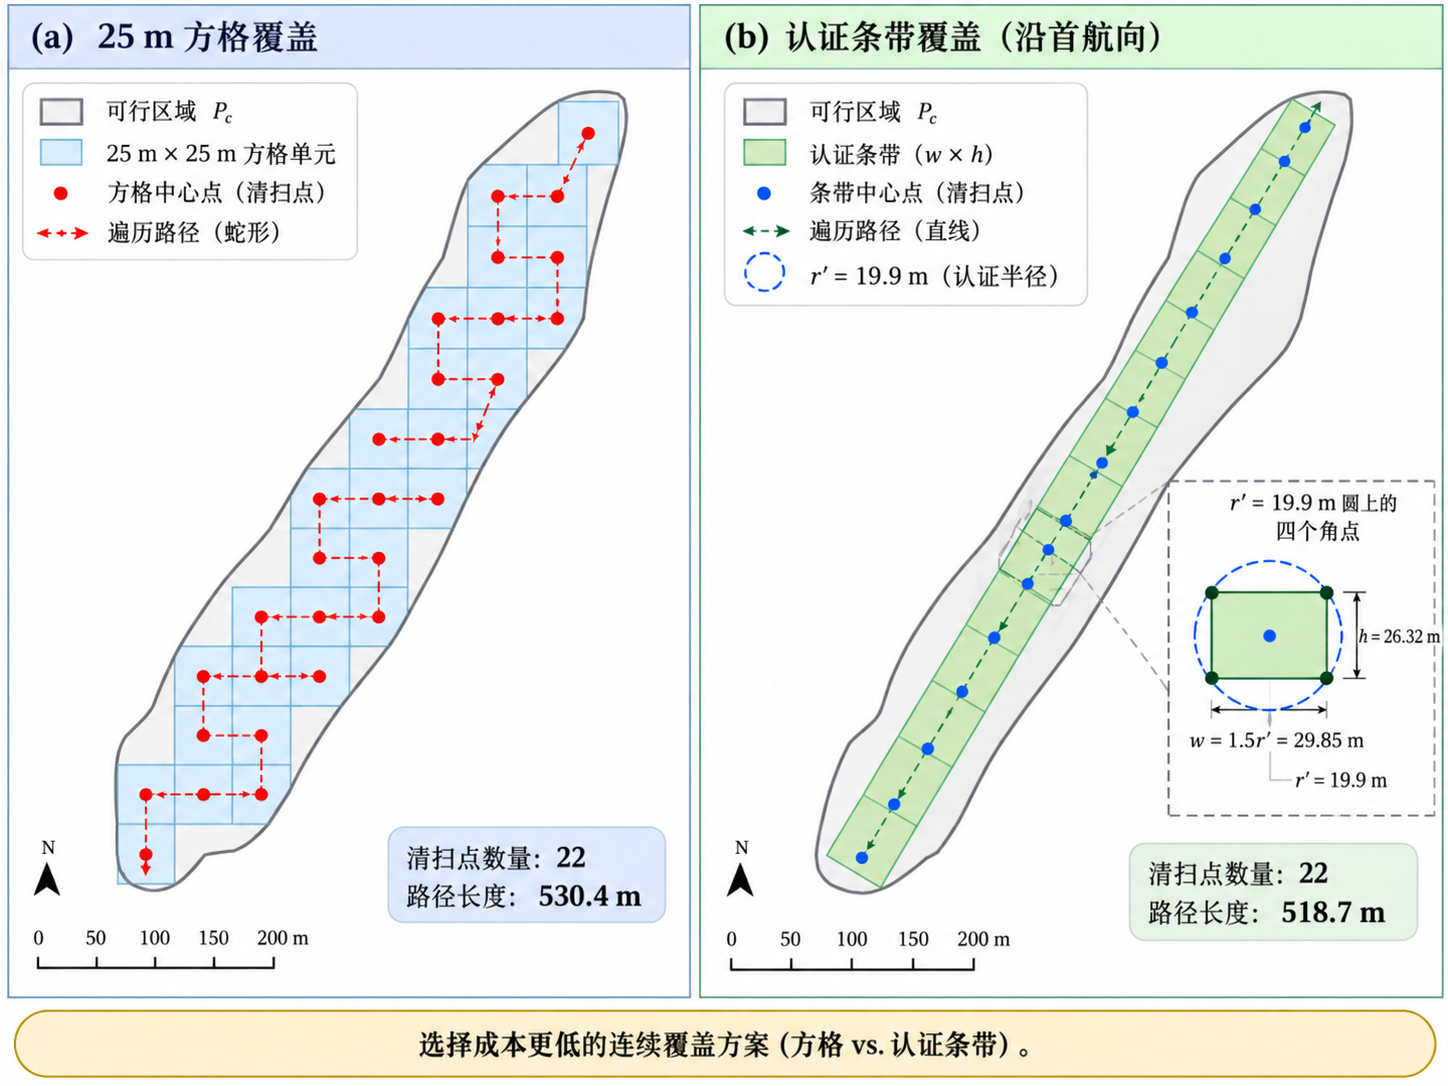
\includegraphics[width=0.9\textwidth]{figures/fig-q4-strip.png}

  \caption{两种具有连续覆盖证明的光学清除点列}\label{fig:q4-strip}
\end{figure}

\paragraph{扫描成本门控与即时清除.} 条带覆盖有时更慢：条带越宽，列数越少但每列越长，路径未必更短。因此算法同时生成方格路线与各个 $w$ 对应的条带路线，按
\begin{equation}\label{eq:routecost}
  \widehat C_{\rm route}=\frac{\|x_1-p_{\rm cur}\|+\sum_{i}\|x_{i+1}-x_i\|}{v}+|\{x_i\}|\cdot t_f
\end{equation}
取其中最小者。同样的比较也用在补测决策上：若估计的光学覆盖成本已不高于“走到补测点再测一次”的成本，就直接进入光学清除，跳过价值不足的补测。最后，收到 \texttt{near} 时在当前测站立即清除，而不等到本站扫描结束——真源就在 $5\mmet$ 之内，任何推迟只会增加往返。

\subsection{实验结果}

第四问历次结构性改进的配对实验见附录~\ref{app:sens}的表~\ref{tab:q4paired}，最后一次布局升级（$25\to22$ 站）的留出验证见\cref{tab:q4holdout}。

\begin{table}[!htbp]
  \caption{$25$ 站 $\to$ $22$ 站的留出验证（新种子 $2026100000$ 起，与全部开发种子不重叠；$220$ 例全部清除）}
  \label{tab:q4holdout}\centering
  \begin{tabular}{lcccccc}
    \toprule[1.5pt]
    场景 & 案例数 & $25$ 站均值 & $22$ 站均值 & $25$ 站 $\mathrm{P}_{95}$ & $22$ 站 $\mathrm{P}_{95}$ & $22$ 站更快 \\
    \midrule[1pt]
    随机       & $100$ & $494.5$ & $478.4$ & $675.5$ & $659.6$ & $73/100$ \\
    边界向外   & $30$  & $588.7$ & $557.9$ & $725.5$ & $683.8$ & $24/30$ \\
    最小接收半径 & $30$ & $517.0$ & $502.7$ & $677.0$ & $611.1$ & $20/30$ \\
    全部定向   & $30$  & $606.1$ & $574.9$ & $776.5$ & $726.3$ & $26/30$ \\
    圆心聚集   & $30$  & $450.9$ & $431.1$ & $598.2$ & $568.8$ & $28/30$ \\
    \bottomrule[1.5pt]
  \end{tabular}\\[2pt]
  \footnotesize 按源数分层（随机集）：$10$ 源 $666\to642$，$13$ 源 $491\to475$，$16$ 源 $361\to346$（虚拟秒/源）。
\end{table}



\cref{tab:q4holdout}显示 $22$ 站在五类场景的均值与 $\mathrm{P}_{95}$ 上都优于 $25$ 站，最困难的“边界向外”“全部定向”改善最明显（$30.8$ 与 $31.2\msec/$源）；但逐例表现有涨有跌，个别案例因发现顺序改变而变慢。本文保留的是“均值与分位数改善、清除率保持 $100\%$”这一较弱但站得住的结论（典型局轨迹与逐例配对见\cref{fig:q4-track}）。

\begin{figure}[!htbp]
  \centering
  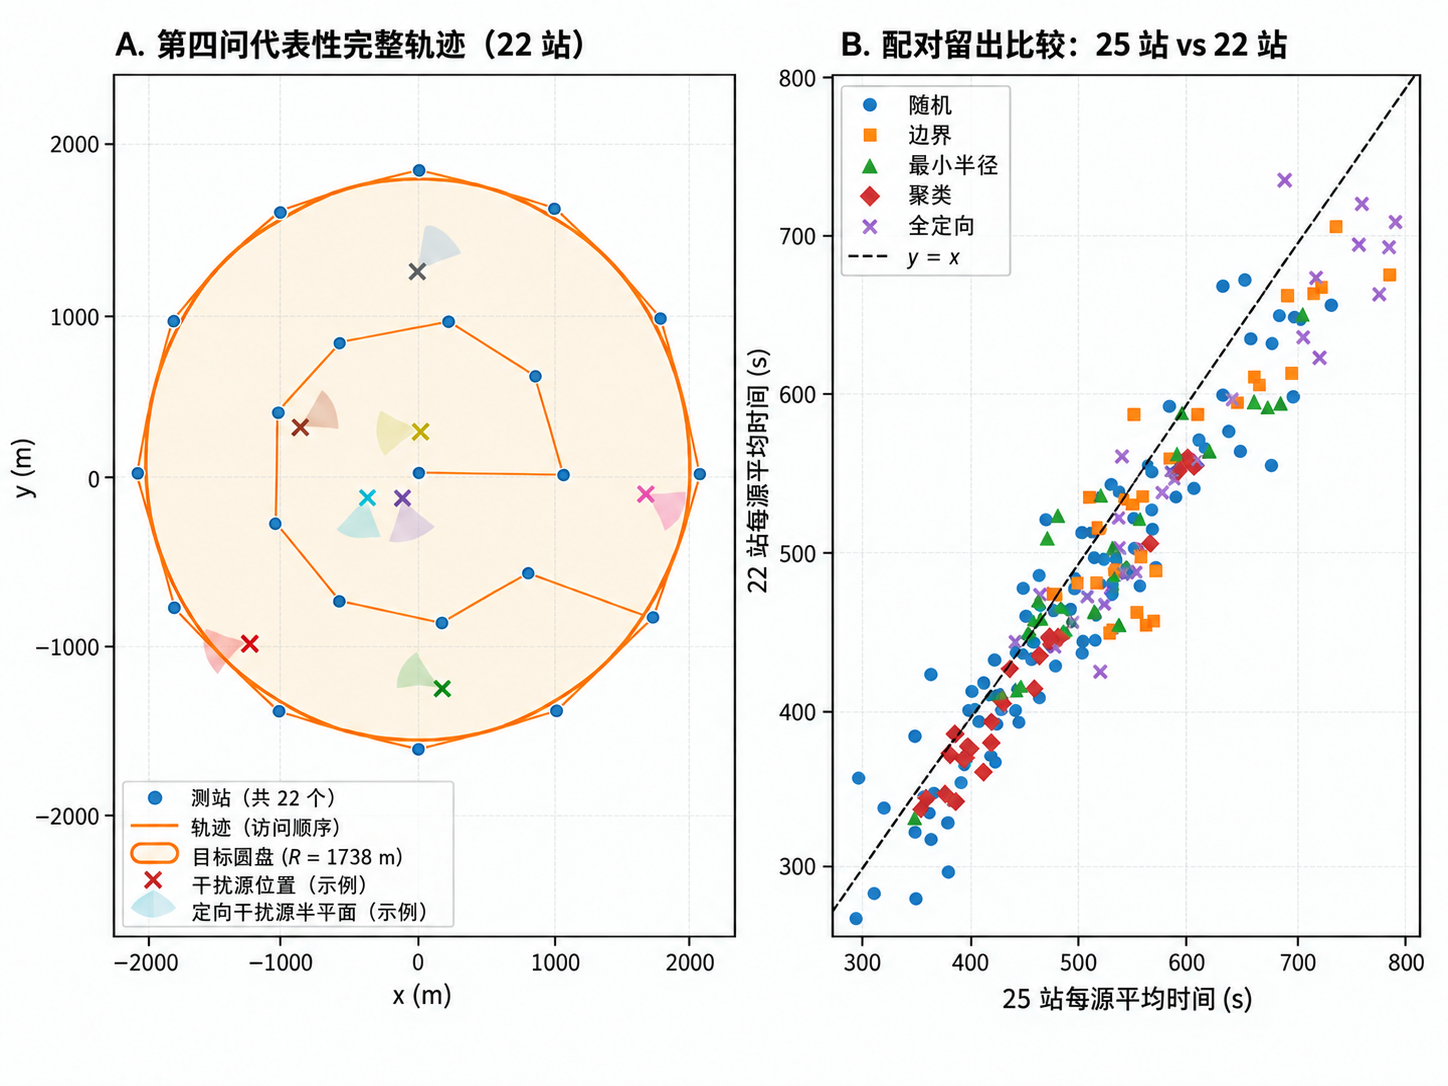
\includegraphics[width=0.9\textwidth]{figures/fig-q4-track.png}
  \caption{第四问典型局的行走轨迹与 $25$ 站／$22$ 站逐例配对}\label{fig:q4-track}
\end{figure}

\subsection{被否决的改进路线}

本文另试过七条改进路线（绕行代价阈值调度、价值门控裁剪重复测量、运行时动态跳站等），均完成完整配对实验但未获稳定收益，完整记录见附录~\ref{app:ablation}的\cref{tab:q4reject}。反复出现的教训是：\textbf{只盯着某个局部指标做优化，往往会在别处付出更大代价。}

\subsection{成本基准与“放弃保证”的代价}\label{sec:q4:lb}

把巡站、全站扫描与到达清除三项相加，得到第四问的成本基准；按源数分层，官方演练比该基准高 $6\%\sim11\%$。需要强调这是一个经验构造，用于判断“现有方案是否已接近一条合理的成本底线”。若放弃覆盖保证，用 $40$ 万个随机定向源做蒙特卡洛估计：$16$ 站时每局期望漏检 $0.14$ 个，约七局就有一局清除率低于 $100\%$；按“清除率是硬约束”的准则，这些方案一律不采用。完整的基准公式、分层表与风险表见附录~\ref{app:fixed}。

\paragraph{本问小结.} $22$ 站布局通过细／粗两次凸包检查，$220$ 例留出与 $70$ 局演练全部清除。需强调：\textbf{$22$ 是本文找到并认证过的最小站数}（其最优性尚未证明）。

\section{演练测试与正式测试结果}\label{sec:results}

\subsection{测试环境与客户端}

机器狗程序用 Python 实现，通过 HTTP$+$JSON 与官方模拟器通信。客户端遵守附件 2 的全部要求：以参赛队号作为 \texttt{robot\_id}，每个新动作使用新的 \texttt{request\_id}，\textbf{串行发送、逐次等待响应}，网络中断后重试时复用原请求内容与原 \texttt{request\_id}；结果未知的动作标记为 \texttt{uncertain} 并禁止发出不同的后续动作，以免重复计时或状态错位。客户端按 \texttt{/enter} 返回的剩余时长设置现实截止时间，并同步记录逐动作日志、配置哈希与定位证书，供事后核对。

\subsection{演练样本的选取规则}

演练测试不限次数，因此日志中混有不同算法版本的记录。为避免把旧版本的成绩算进当前方案，本文按三条规则筛选样本，规则在看到成绩之前就已固定：

\begin{enumerate}[label=(\arabic*),itemsep=1pt]
  \item 该局状态为 \texttt{completed} 且由机器狗\textbf{主动调用 \texttt{/exit}} 结束——中途失败、超时或被手工中止的记录一律剔除；
  \item 该局所用的策略源码哈希与当前提交版本一致（第三问 \texttt{d12fa3a5}，第四问 \texttt{3de0e9a0}）；
  \item 该局所用的配置与当前默认配置逐项一致。
\end{enumerate}

按此规则，第三问保留 $50$ 局、第四问保留 $70$ 局；另有 $25$ 局第三问记录因补测精化的参数与当前配置不同而被排除，排除清单与原因随支撑材料一并给出。\textbf{没有任何一局因为成绩不好而被剔除。}

\subsection{演练测试结果}

演练结束后模拟器界面会显示本局干扰源总数，逐局核对表明它与机器狗的成功清除数完全一致，故
\begin{equation}
  \text{被清除干扰源个数的比例}=\frac{N_c}{n}=100\%\quad\text{（全部 }120\text{ 局）} .
\end{equation}
汇总结果见\cref{tab:practice-summary}，按源数分层的结果见\cref{tab:practice-strat}。逐局明细（含每局的时间分项与动作数）见支撑材料 \texttt{q3\_runs.csv} 与 \texttt{q4\_runs.csv}。

\begin{table}[!htbp]
  \caption{官方模拟器演练测试汇总（时间单位：虚拟秒）}\label{tab:practice-summary}\centering\small
  \begin{tabular}{lcc@{\hspace{2em}}lcc}
    \toprule[1.5pt]
    指标 & 问题三 & 问题四 & 指标 & 问题三 & 问题四 \\
    \midrule[1pt]
    有效局数 & $50$ & $70$ & 平均 s/源（案例口径） & $252.0$ & $511.2$ \\
    清除源总数 & $667$ & $887$ & 平均 s/源（合并口径） & $247.5$ & $500.2$ \\
    清除比例 & $100\%$ & $100\%$ & 标准差／中位数 & $34.3$／$251.5$ & $83.7$／$515.8$ \\
    整局总时间均值 & $3301$ & $6338$ & 四分位区间 & $226.6\sim279.4$ & $445.7\sim563.9$ \\
    \quad 标准差／变异系数 & $291$／$8.8\%$ & $398$／$6.3\%$ & $\mathrm{P}_{95}$ & $301.6$ & $644.6$ \\
    动作数 & $127\sim201$ & $187\sim390$ & 最好／最差 & $185.2$／$314.8$ & $340.6$／$681.7$ \\
    程序运行时间/s & $0.4\sim2.2$ & $0.7\sim1.1$ & 清满 $16$ 源提前结束 & $5$ 局 & $3$ 局 \\
    \bottomrule[1.5pt]
  \end{tabular}
\end{table}

\begin{table}[!htbp]
  \caption{演练成绩按源数分层（平均定位清除时间，案例口径，虚拟秒/源）}\label{tab:practice-strat}\centering
  \begin{tabular}{lccccccc}
    \toprule[1.5pt]
    源数 $n$ & $10$ & $11$ & $12$ & $13$ & $14$ & $15$ & $16$ \\
    \midrule[1pt]
    问题三：局数 & $3$ & $12$ & $5$ & $7$ & $4$ & $6$ & $13$ \\
    \qquad\ \ 均值 & $296.4$ & $282.1$ & $277.9$ & $259.5$ & $247.5$ & $215.2$ & $218.3$ \\
    问题四：局数 & $10$ & $11$ & $13$ & $12$ & $10$ & $10$ & $4$ \\
    \qquad\ \ 均值 & $639.3$ & $575.5$ & $537.1$ & $494.7$ & $445.3$ & $418.8$ & $375.2$ \\
    \bottomrule[1.5pt]
  \end{tabular}
\end{table}

两张表合起来印证了\cref{sec:analysis:fixed}的判断。整局虚拟总时间的变异系数只有 $6\%\sim9\%$，而平均定位清除时间在 $n=10$ 与 $n=16$ 之间相差 $78\msec/$源（第三问）与 $264\msec/$源（第四问）——\textbf{波动几乎全部来自分母，而不是算法本身不稳定}。第四问 $70$ 局中有 $3$ 局在访问完 $19$ 或 $21$ 站时就清满 $16$ 个源而提前退出，这也是其总时间随源数轻微\emph{下降}的原因。

\subsection{本地模型与官方模拟器的一致性}

本文所有版本比较都在本地合成模拟器上完成，因此本地环境与官方环境的差距直接关系到这些结论能否外推。把\cref{tab:q4holdout}脚注中的本地留出分层预测与官方演练的同源数结果对照，得到\cref{tab:q4match}。

\begin{table}[!htbp]
  \caption{问题四本地留出预测与官方演练的分层对照（虚拟秒/源）}\label{tab:q4match}\centering
  \begin{tabular}{ccccc}
    \toprule[1.5pt]
    源数 $n$ & 本地留出预测 & 官方局数 & 官方实测 & 官方比本地 \\
    \midrule[1pt]
    $10$ & $642$ & $10$ & $639.3$ & $-0.4\%$ \\
    $13$ & $475$ & $12$ & $494.7$ & $+4.1\%$ \\
    $16$ & $346$ & $4$  & $375.2$ & $+8.4\%$ \\
    \bottomrule[1.5pt]
  \end{tabular}
\end{table}

两者在量级上吻合，但存在一个系统性趋势：\textbf{源数越多，官方环境比本地慢得越明显}，偏差从 $-0.4\%$ 升到 $+8.4\%$。一个合理的解释是官方案例中源的空间分布比本地采用的面积均匀分布更分散，使多目标之间顺路共享观测的机会变少；不过 $n=16$ 只有 $4$ 局，这一趋势本身也可能只是抽样噪声。

因此本文对这一比较只作如下有限的表述：\emph{在已有 $70$ 局官方演练覆盖的源数范围内，本地模型与官方模拟器给出的耗时量级一致，本地配对实验中“甲版本快于乙版本”这类定性结论可以谨慎外推。}它既不足以证明两种案例的分布相同，也不保证正式测试中同样的相对收益一定成立。

\begin{figure}[!htbp]
  \centering

  %% 画法建议：三个子图。(a) 散点图：横轴源数 $n$、纵轴整局虚拟总时间，第三问与第四问分别用不同颜色，
  %% 叠加回归直线 $T_{Q3}=2396+68n$、$T_{Q4}=6848-40n$ 及其 $95\%$ 带（数据取自 \texttt{q3\_runs.csv}、\texttt{q4\_runs.csv}，共 $50+70$ 点），
  %% 直观展示“总时间主要由固定成本决定”；第四问的回归线近乎水平甚至微降，可加注 $r=-0.18$。
  %% (b) 同样的横轴、纵轴改为平均定位清除时间 $\bar T$，画出 $120$ 个散点、按源数分组的箱线图，
  %% 并叠加双曲线 $\bar T=T_0/n+k$，说明分母效应。
  %% (c) 堆叠柱状图：第三问与第四问的每源时间构成（移动／检测／切频／光学定位／激光），数据取自\cref{tab:breakdown}。
  \fbox{\parbox[c][2.2cm][c]{0.86\textwidth}{\centering\small
  【待插图】（绘图要求见本段 \TeX{} 源码注释）}}
  \caption{演练成绩随源数的变化与时间构成}\label{fig:results}
\end{figure}

\cref{fig:results}把两问 $120$ 局演练成绩按源数与时间构成做了汇总。

\subsection{正式测试结果}

三次正式测试的结果分别按题目表 1 的格式列于\cref{tab:formal3}与\cref{tab:formal4}。

%%%%%%%%%%%%%%%%%%%%%%%%%%%%%%%%%%%%%%%%%%%%%%%%%%%%%%%%%%%%%%%%%%%%%%%%%%%%%%%%
%% TODO（提交前必改）：以下两张表在完成三次正式测试后按模拟器界面填写。
%%   1. 测试案例编码：直接抄模拟器界面显示的编码，不要改写。
%%   2. 清除干扰源个数：取 practice_logs/<局>/summary.json 的 cleared_count。
%%   3. 平均定位清除时间：取 average_per_cleared_s（= total_virtual_s / cleared_count）。
%%   4. 程序运行时间：取 program_elapsed_s（/enter 到测试结束的现实时长）。
%%   5. 填完后删除下面这一段 \noindent\fbox{...} 提示文字。
%%   6. 导出三次正式测试的加密日志（不要改文件名）放入支撑材料。
%%%%%%%%%%%%%%%%%%%%%%%%%%%%%%%%%%%%%%%%%%%%%%%%%%%%%%%%%%%%%%%%%%%%%%%%%%%%%%%%
\noindent\fbox{\parbox{\dimexpr\linewidth-14pt\relax}{\small\textbf{【待填写】}三次正式测试完成后，按模拟器界面的测试案例编码与本地
\texttt{summary.json} 中的 \texttt{cleared\_count}、\texttt{average\_per\_cleared\_s}、\texttt{program\_elapsed\_s}
填入下列两表，并删除本提示框。}}\medskip

\begin{table}[!htbp]
  \caption{问题三正式测试结果}\label{tab:formal3}\centering
  \begin{tabular}{cccc}
    \toprule[1.5pt]
    测试案例编码 & 清除干扰源个数 & 平均定位清除时间/s & 程序运行时间/s \\
    \midrule[1pt]
    测试 $1$ 案例编码 &  &  &  \\
    测试 $2$ 案例编码 &  &  &  \\
    测试 $3$ 案例编码 &  &  &  \\
    \bottomrule[1.5pt]
  \end{tabular}
\end{table}

\begin{table}[!htbp]
  \caption{问题四正式测试结果}\label{tab:formal4}\centering
  \begin{tabular}{cccc}
    \toprule[1.5pt]
    测试案例编码 & 清除干扰源个数 & 平均定位清除时间/s & 程序运行时间/s \\
    \midrule[1pt]
    测试 $1$ 案例编码 &  &  &  \\
    测试 $2$ 案例编码 &  &  &  \\
    测试 $3$ 案例编码 &  &  &  \\
    \bottomrule[1.5pt]
  \end{tabular}
\end{table}

\subsection{成绩的正确解读}

三次正式测试是三个独立随机案例，样本量极小，因此有必要先说清楚成绩该怎么读。\textbf{第一，三次成绩的差异主要由抽到的源数决定，而不是算法是否稳定}：演练中整局虚拟总时间的变异系数只有 $6\%\sim9\%$，而平均定位清除时间在 $n=10$ 与 $n=16$ 之间相差近一半（\cref{tab:practice-strat}），因此本文同时报告两个指标，解读时优先看整局总时间。\textbf{第二，两种平均口径不能混用}：案例口径与合并口径的定义见\cref{eq:twomeans}，两者相差约 $2\%$，本文所有对比都在同一口径下进行并在表注中标明。\textbf{第三，清除比例排在时间之前}：只有在 $N_c=n$ 时比较 $\bar T$ 才有意义，某局若未清完，$\bar T$ 反而可能因分母变小而“变好”，这类记录必须单列。\textbf{第四，程序运行时间不是效率指标}：它在演练中只有 $0.4\sim2.2\msec$（第三问）与 $0.7\sim1.1\msec$（第四问），相对 $1200\msec$ 的限制有三个数量级余量，主要由 HTTP 往返次数决定，与虚拟时间没有可比性。

\section{模型的检验、灵敏度分析与评价}\label{sec:eval}

\subsection{正确性检验的内容}

本文的每一次实验都包含逐例核验：清除数是否等于真实源数；每次成功清除时清除点到真源的距离是否不超过 $20\mmet$；每一时刻的可行多边形与其最小包围圆是否确实包含真源（即\cref{eq:invariant}）；逐条动作重新累加的时间与日志时钟之差是否在 $10^{-6}\msec$ 以内；测站布局是否在连续域上满足覆盖条件；各类边界与退化几何是否处理正确；候选版本有无退步案例；以及失败运行是否被独立保留。

其中第三项尤其关键。\cref{app:debug}记录的那次失败正是“清除数看似完全正确、几何证书却已经失效”的情形，它说明\textbf{结果正确不意味着不做检查}。

\subsection{灵敏度分析}

\paragraph{对测向误差界的灵敏度.}

改变实际误差幅度、同时把算法的误差界同步放宽为“幅度 $+0.005^\circ$”，每档使用相同的种子，结果见附录~\ref{app:sens}的\cref{tab:senserr}。该组实验做在早期的“两次测向”基线上，只用于观察趋势，其绝对数值不代表当前版本。

误差幅度加倍只带来 $2\%$（问题三）与 $5\%$（问题四）的时间增长，说明在误差界被正确告知的前提下，方案对误差幅度不敏感。原因是：可行域的尺度与 $\bar\varepsilon$ 成正比，但总时间的主体是与 $\bar\varepsilon$ 无关的巡站与扫描固定成本。

\paragraph{对误差的失配是危险的.} 需要强调的是，这种“不敏感”并不意味着方案对误差界的设定可以放松；相反，误差界的失配可能导致可行域被错误裁剪。附录~\ref{app:sens}的表~\ref{tab:senserr}只说明“正确知道更大误差界”时的灵敏度。本文专门构造了真实偏差达 $1.5^\circ$ 而算法只容许 $1.005^\circ$ 的算例，结果出现正的半平面违约 $12.958908\mmet$——真源被排出了可行域，包含性不变量被破坏。这正是算法采用略宽于 $1^\circ$ 的保守界 $\bar\varepsilon=1.005^\circ$ 的原因：吸收“误差先产生、再按两位小数取整”可能带来的额外偏差。一旦正式测试中出现空交集或“认证清除失败”，正确的做法是排查取整、角度约定、坐标与计时，确认无误后再决定是否调整阈值。因此，在误差界能够被正确估计并同步调整的前提下，方案对误差幅度变化总体不敏感。

\paragraph{对最小接收半径的灵敏度.} 这是全文最关键的敏感参数，因为两问的覆盖保证都以 $\rho_{\min}=1000\mmet$ 为前提。第三问相当宽裕：由\cref{thm:hexcover}，七站布局可行当且仅当 $\rho_{\min}\ge R/2=900\mmet$，题设 $1000\mmet$ 有 $11.1\%$ 余量。第四问则薄得多：$22$ 站布局在 $\rho_{\min}\ge994\mmet$ 时仍通过、$990\mmet$ 时失效（附录~\ref{app:sens}表~\ref{tab:sensrho}），容忍度约 $6\sim10\mmet$；表中 $998\sim1000\mmet$ 的余量不变、$994\mmet$ 突降是粗网格量化所致，题设下的真实几何余量以 $h=1\mmet$ 细网格的 $1.7331\mmet$ 为准（\cref{sec:q4:cert}）。值得注意的是，优化搜索得到的 $22$ 站布局不仅比解析的 $25$ 站更快，对 $\rho_{\min}$ 的余量也更大（约 $6\sim10\mmet$ 对不足 $2\mmet$）；两者余量都不宽，故程序保留回退开关：删除配置中的 \texttt{q4\_station\_list} 即恢复 $25$ 站布局。

\paragraph{对光学格距与其他阈值的灵敏度.} 光学兜底要求 $h_{\rm opt}\le28.2843\mmet$（取 $25\mmet$），条带覆盖要求外接圆半径 $\le r_c$（取 $19.9\mmet$），认证阈值取 $20\mmet-10^{-6}$。这些阈值一旦被误改超限，覆盖保证立即失效，因此程序启动时统一校验、不满足即拒绝运行。

\subsection{稳健性（压力场景）}

除随机案例外，本文设计了五类压力场景：源全部贴近区域边界且取最小接收半径、源在圆心聚集、全体取最小接收半径、第四问全部为朝外的定向源、固定 $\pm1^\circ$ 偏差与光滑空间相关偏差。\cref{tab:q4holdout}给出了第四问五类场景的完整结果：$220$ 例全部清除，$22$ 站在每一类上都优于 $25$ 站。第三问的压力集（$70$ 例、$890$ 源）同样全部清除，只有 $2$ 例轻微退步，最大退步 $2.72\msec/$源。

\subsection{模型的优点}

\textbf{核心贡献有四点。第一，“一定能清完”是一条可证明的性质}：\cref{thm:term3}与\cref{thm:hull}把终止条件建立在连续域几何覆盖上，\cref{thm:cert}把它化为可执行的有限检查，\cref{cor:certify}与\cref{eq:grid}、\cref{eq:strip}保证清除动作确定性成功，整条链路上没有一步靠“试几次收不到就认为没有”。\textbf{第二，七站达到距离覆盖的理论下界}：\cref{thm:seven}证明 $6$ 站不可能、$7$ 站可达。\textbf{第三，凸包条件刻画定向源的方向覆盖，$22$ 站取得连续域证书}：该布局在 $1018.68$ 万点细网格上最小余量 $1.7331\mmet$，所比较布局中 $\le21$ 站均无法通过。\textbf{第四，时间诊断驱动布局优化}：先由\cref{sec:analysis:fixed}认定固定成本主导，再把优化落到测站布局上。此外，题目只给出误差的界，本文据此只用凸多边形交与最小包围圆，并对所有近似取保守外包，使包含性不变量单调成立。

\textbf{工程优化另有若干}：\texttt{no\_signal} 圆盘排除、认证条带覆盖、共享测站扫描、圆心补测精化、有界等待与即时清除等，贯穿第\ref{sec:q3}、\ref{sec:q4}节。附录~\ref{app:ablation}的表~\ref{tab:q3reject}与表~\ref{tab:q4reject}保留了 $11$ 条被否决的路线与一次几何证书失效，它们既是消融实验，也是结论可信度的一部分；覆盖保证参数在程序启动时统一校验，不满足即拒绝运行。

\subsection{模型的缺点与局限}

\begin{enumerate}[label=(\arabic*),itemsep=1pt]
  \item \textbf{调度层是启发式的.} 混合贪心只比较一步的移动代价，没有纳入未来的测量结果与光学路径；两步前瞻的尝试反而更慢（\cref{tab:q3reject}），但这不说明贪心已最优。
  \item 第四问的 \texttt{no\_signal} 尚未被利用. 一次“收不到”蕴含“距离超限或背向”的析取信息，可在“位置 $\times$ 朝向”的联合状态空间上做保守排除；本文原型未能胜过现行方案，这是最有价值的未完成方向。
  \item \textbf{覆盖余量偏薄.} $22$ 站布局对 $\rho_{\min}$ 只有约 $6\sim10\mmet$ 的余量（\cref{tab:sensrho}）；若官方对 $\rho_{\min}$ 的保证比 $1000\mmet$ 更弱，覆盖可能失效。
  \item \textbf{本地分布未必与官方一致.} \cref{tab:q4match}显示偏差随源数从 $-0.4\%$ 升到 $+8.4\%$，故本地配对实验的相对结论可谨慎外推、绝对数值不能。
  \item \textbf{异常只能安全停止.} 客户端会检测超时与协议异常、记录现场并停在原地退出，但没有自动恢复能力。
  \item \textbf{结论依赖题设的理想化物理.} 静止源、无遮挡直线行走、确定性阈值、误差有界，任一被打破，包含性不变量与覆盖证明都需重建。
\end{enumerate}

\subsection{模型的改进与推广}

针对上述局限，最值得推进的是把 \texttt{no\_signal} 的析取信息纳入“位置 $\times$ 朝向”的联合证书，并在多机协同下进一步摊薄固定成本。本文框架也可推广：区域改变时只需把\cref{thm:cert}的网格证书套用到新区域重新搜索布局；定向覆盖角收窄为 $2\beta$ 时把凸包条件换成更强的“任意 $\beta$-锥内至少有一站”；多机协同则化为测站集划分的 min--max $k$-TSP。水下声源搜寻、林区火点定位等“方位有界误差、作用距离有下界、处置有作用半径”的任务也可整体移植。

最后需要说明：本文的工程价值不仅在于给出一个可运行的方案，更在于区分了严格保证、数值验证与经验估计三类结论。


\CumcmAIUsed{语言润色与表述打磨、\LaTeX{} 排版与公式规范化、以及程序语法层面的调试；问题的分析、建模、定理证明、算法设计与全部实验均由参赛队员独立完成}

\begin{thebibliography}{9}
  \bibitem{bezdek} K.~Bezdek.
  \newblock \"{U}ber einige Kreis\"{u}berdeckungen [J].
  \newblock \emph{Beitr\"{a}ge zur Algebra und Geometrie}, 1983, 14: 7--13.
  \bibitem{bezdek2} K.~Bezdek.
  \newblock \"{U}ber einige optimale Konfigurationen von Kreisen [J].
  \newblock \emph{Ann. Univ. Sci. Budapest. E\"{o}tv\"{o}s Sect. Math.}, 1984, 27: 143--151.
  \bibitem{jung} H.~W.~E.~Jung.
  \newblock \"{U}ber die kleinste Kugel, die eine r\"{a}umliche Figur einschlie{\ss}t [J].
  \newblock \emph{Journal f\"{u}r die reine und angewandte Mathematik}, 1901, 123: 241--257.
  \bibitem{welzl} E.~Welzl.
  \newblock Smallest enclosing disks (balls and ellipsoids) [M].
  \newblock \emph{New Results and New Trends in Computer Science}, LNCS 555, Springer, 1991: 359--370.
  \bibitem{bhh} J.~Beardwood, J.~H.~Halton, J.~M.~Hammersley.
  \newblock The shortest path through many points [J].
  \newblock \emph{Mathematical Proceedings of the Cambridge Philosophical Society}, 1959, 55(4): 299--327.
  \bibitem{rockafellar} R.~T.~Rockafellar.
  \newblock \emph{Convex Analysis} [M].
  \newblock Princeton University Press, 1970.
  \bibitem{toth} G.~Fejes T\'{o}th.
  \newblock Thinnest covering of a circle by eight, nine, or ten congruent circles [J].
  \newblock \emph{Combinatorial and Computational Geometry}, MSRI Publications 52, 2005: 361--376.
  \bibitem{torrieri} D.~J.~Torrieri.
  \newblock Statistical theory of passive location systems [J].
  \newblock \emph{IEEE Transactions on Aerospace and Electronic Systems}, 1984, AES-20(2): 183--198.
  \bibitem{cumcm2026} 2026 年高教社杯全国大学生数学建模竞赛 B 题《无线电干扰源的快速自动定位与清除》及附件 1、附件 2.
  \bibitem{kaelbling} L.~P.~Kaelbling, M.~L.~Littman, A.~R.~Cassandra.
  \newblock Planning and acting in partially observable stochastic domains [J].
  \newblock \emph{Artificial Intelligence}, 1998, 101(1--2): 99--134.
  \bibitem{milanese} M.~Milanese, A.~Vicino.
  \newblock Optimal estimation theory for dynamic systems with set membership uncertainty: an overview [J].
  \newblock \emph{Automatica}, 1991, 27(6): 997--1009.
  \bibitem{kershner} R.~Kershner.
  \newblock The number of circles covering a set [J].
  \newblock \emph{American Journal of Mathematics}, 1939, 61(3): 665--671.
\end{thebibliography}

\newpage
\begin{appendices}

\section{支撑材料清单}

\begin{table}[!htbp]
  \caption{支撑材料目录说明}\centering
  \begin{tabularx}{\textwidth}{>{\raggedright\arraybackslash}p{4.6cm} L}
    \toprule[1.5pt]
    文件／目录 & 内容 \\
    \midrule[1pt]
    \texttt{code/model.py} & 有界误差几何：楔形半平面、多边形裁剪、半平面交的空／无界／有界判定、直径、最小包围圆、光学格、测站布局生成与覆盖校验 \\
    \texttt{code/optimized.py} & 在线策略主体：轨迹维护、共享测站扫描、认证清除与光学兜底入口 \\
    \texttt{code/q3\_policy.py} & 第三问专用：目标圆外切约束、\texttt{no\_signal} 圆盘排除、第二测点、圆心补测、混合贪心调度 \\
    \texttt{code/q4\_policy.py} & 第四问专用：$22$ 站列表校验与凸包方向覆盖检查、选择性重测、有界等待、补测精化、条带清除 \\
    \texttt{code/q4\_optical.py} & 认证条带覆盖与扫描路线成本比较 \\
    \texttt{code/\allowbreak practice\_robot.py} & 官方模拟器 HTTP 客户端：串行发送、超时原样重试、未决动作保护、逐动作日志与预算控制 \\
    \texttt{code/config.json} & 当前全部算法参数与 $22$ 站坐标 \\
    \texttt{code/layout\_opt.py}、\allowbreak\texttt{code/certify22.py} & 方向覆盖余量计算与 $h=1\mmet$ 网格证书 \\
    \texttt{official\_practice/} & 演练样本：\texttt{q3\_runs.csv}、\texttt{q4\_runs.csv} 为 $50+70$ 局的逐局明细，
      \texttt{official\_runs.json} 另含被排除记录的清单与原因 \\
    \texttt{logs/}（三次正式测试） & 模拟器导出的加密行为日志，文件名未作任何修改 \\
    \texttt{AI工具使用详情.pdf} & 按 2026 年 AI 工具使用规定提交的详情说明 \\
    \bottomrule[1.5pt]
  \end{tabularx}
\end{table}

\noindent 运行方式：安装 Python 3.10 及以上与 \texttt{numpy}、\texttt{scipy}、\texttt{requests}，在模拟器接口就绪后执行
\begin{center}
\texttt{python practice\_robot.py --question 3 --robot-id <队号> --case-code <案例编码> --connect}
\end{center}
（第四问将 \texttt{--question} 改为 \texttt{4}）。不加 \texttt{--connect} 时程序不会发送任何请求，便于离线检查。

\section{关键参数配置}

\begin{table}[!htbp]
  \caption{算法参数及其来源}\centering\small
  \begin{tabularx}{\textwidth}{@{}l l L l@{}}
    \toprule[1.5pt]
    参数 & 取值 & 作用 & 来源 \\
    \midrule[1pt]
    \texttt{region\_radius\_m}        & $1800$   & 目标区域半径 & 题目 \\
    \texttt{receiver\_radius\_min\_m} & $1000$   & 接收半径下界，覆盖证明的基准 & 题目 \\
    \texttt{receiver\_radius\_max\_m} & $1500$   & 接收半径上界，初始楔形长度 & 题目 \\
    \texttt{bearing\_bound\_deg}      & $1.005$  & 保守误差界 & \cref{asu:bounded} \\
    \texttt{clear\_m}                 & $20$     & 认证清除半径 & 题目 \\
    \texttt{near\_m}                  & $5$      & 近场阈值 & 题目 \\
    \texttt{optical\_grid\_m}         & $25$     & 光学方格边长，$25/\sqrt2<20$ & \cref{eq:grid} \\
    \texttt{q3\_survey\_layout}       & hexagon  & 第三问七站布局 & \cref{thm:seven} \\
    \texttt{q3\_ring\_radius\_m}      & $1150$   & 第三问环半径，可行区间 $[1122.96,1732.05]$ & \cref{cor:ring} \\
    \texttt{q3\_policy}               & mixed    & 搜索与目标混合贪心调度 & \cref{sec:q3:shared} \\
    \texttt{q3\_second\_forward/lateral\_m} & $200$／$100$ & 第二测点偏移 & \cref{sec:q2} \\
    \texttt{q3\_refine\_max\_m}       & $300$    & 圆心补测的适用上限 & \cref{sec:q3:refine} \\
    \texttt{q3\_refine\_offset\_m}    & $60$     & 补测横移距离 & \cref{sec:q3:refine} \\
    \texttt{q4\_policy}               & mixed\_ring & 第四问联合调度 & \cref{sec:q4:online} \\
    \texttt{q4\_station\_list}        & $22$ 点  & 认证布局，删除即回退 $25$ 站 & \cref{tab:q4layout} \\
    \texttt{q4\_selective\_remeasure} & true     & 选择性重测 & \cref{eq:selective} \\
    \texttt{q4\_remeasure\_min\_sine} & $0.3$    & 重测的最小交会角正弦 & \cref{eq:selective} \\
    \texttt{q4\_remeasure\_min\_gap\_m}& $300$   & 重测的最小测点间距 & \cref{eq:selective} \\
    \texttt{q4\_station\_help\_m}     & $950$    & 判定测站对目标是否有价值 & \cref{eq:selective} \\
    \texttt{q4\_wait\_for\_survey}／\texttt{q4\_wait\_mode} & true／inner & 有界等待，仅限内环发现的目标 & \cref{sec:q4:online} \\
    \texttt{q4\_wait\_stale\_m}       & $1400$   & 超过该距离不再等待 & \cref{sec:q4:online} \\
    \texttt{q4\_refine\_max\_m}       & $150$    & 第四问补测的适用上限 & \cref{sec:q4:online} \\
    \texttt{q4\_strip\_cover}         & true     & 认证条带覆盖 & \cref{eq:strip} \\
    \texttt{q4\_scan\_cost\_gate}     & true     & 扫描成本门控 & \cref{eq:routecost} \\
    \texttt{q4\_immediate\_near}      & true     & 收到 \texttt{near} 立即清除 & \cref{sec:q4:online} \\
    \bottomrule[1.5pt]
  \end{tabularx}\\[2pt]
  \footnotesize \texttt{config.json} 中另有若干历史参数（如通用的 \texttt{second\_forward\_m}$=650$、\texttt{second\_lateral\_m}$=250$
  以及 \texttt{q3\_grid\_m}、\texttt{q4\_grid\_m}、\texttt{q4\_triangle\_spacing\_m}）。它们\textbf{不被当前默认路径读取}：
  第三、四问的第二测点分别取 \texttt{q3\_}、\texttt{q4\_} 前缀的同名参数。保留这些条目是为了能一键回退到历史对照版本
  （例如置 \texttt{q3\_policy=legacy} 或删除 \texttt{q4\_station\_list}），复现旧轮次实验时仍需要它们，因此没有删除。
\end{table}

\section{调试记录：一次边界顶点的浮点失稳}\label{app:debug}

在第三问圆盘排除约束的首轮验证中，种子 $2031091108$ 的案例报出
\texttt{Localization certificate excluded true source by 9.7374 m}：该局虽然最终清除了全部 $15$ 个源，但中间的几何证书已经失效。根因是重复施加圆盘排除时，一个理论上位于边界的交点被浮点判为落在圆盘内部，相应二次方程的根又略微超出线段参数范围，导致边界顶点被错误丢弃，多次裁剪后可行域出现不保守的收缩。修复后改用平方距离容差保留边界顶点、对接近端点的根做范围容许与夹取、点数不足或凸包退化时保留输入多边形，并补充了重复约束的回归测试。本例说明“结果全部清除”不能替代对中间几何不变量的检查（正文\cref{sec:q3:loc}）。

\section{虚拟时间上界的推导}\label{app:bound}

所有行动点都在以原点为心、$2000\mmet$ 为半径的圆内，任意两点距离不超过 $4000\mmet$。$7$ 个测站每站至多 $20$ 次含切频的检测（$120\msec$）；至多 $16$ 个目标，每个目标至多两段全局跳转、一条保守长度 $6500\mmet$ 的光学路线、若干次检测与至多 $183$ 次清除尝试\footnote{$2000\mmet$：最外环测站半径 $1150\mmet$（第三问）与 $1866\mmet$（第四问）均不超过 $1866\mmet$，而所有源都在 $R=1800\mmet$ 内，第二测点与光学格点也仅在其附近，故所有行动点到原点的距离不超过 $2000\mmet$。$6500\mmet$：对任意“交会后凸子集”，按 $25\mmet$ 方格的列式蛇形路线，每列内部移动不超过 $50\mmet$，相邻非空列间距不超过 $\sqrt{25^2+50^2}\mmet$，且连续凸域不会跳过内部列，故单目标光学路径以 $6500\mmet$ 为上界。$183$：在 $\bar\varepsilon=1.005^\circ$、格距 $25\mmet$ 下，单个可行域的候选格中心至多 $61$ 个横向列 $\times3$ 个纵向行 $=183$ 格。三者均按最坏情形取保守上界，只用于确认 $T$ 远小于虚拟时间上限，不参与任何决策。}。于是
\begin{equation}
  T\le 7\Bigl(\frac{4000}{5}+120\Bigr)+16\Bigl[\frac{2\times4000+6500}{5}+6\times6+183\times3+5\Bigr]
  \approx6.2\times10^{4}\msec\ \ll\ 3.6\times10^{5}\msec,
\end{equation}
远小于虚拟时间上限，也说明算法不可能因死循环而被强制终止。实际演练中整局虚拟时间为 $3301\pm291\msec$，第三问的现实程序运行时间仅 $0.4\sim2.2\msec$，相对 $1200\msec$ 的限制有三个数量级的余量。


\section{被否决改进路线的完整记录}\label{app:ablation}

下列两表汇总了第三、四问中完成了完整配对实验、但最终未进入正式方案的全部改进路线。每一行都使用与开发阶段不重叠的留出案例、同一误差场做配对比较，清除率均为 $100\%$。保留这些记录的目的有两个：它们构成本文的消融实验，说明最终算法的每一项选择都有对照；同时也提醒读者，平均值改善并不足以作为采用一项改动的充分理由。

\begin{table}[!htbp]
  \caption{第三问被否决的改进方案（均完成完整配对实验，清除率均为 $100\%$）}\label{tab:q3reject}\centering
  \begin{tabularx}{\textwidth}{>{\raggedright\arraybackslash}p{4.4cm} c c L}
    \toprule[1.5pt]
    方案 & 对照 s/源 & 候选 s/源 & 否决原因 \\
    \midrule[1pt]
    两步前瞻调度：选动作时同时计入下一步的最优代价，$J(a)=C(p,a)+\lambda\min_bC(a,b)$ & $263.920$ & $292.795$ & 总移动距离由 $12583$ 升至 $14452\mmet$，$\mathrm{P}_{95}$ 同步恶化；复杂度上升而性能下降 \\
    非凸可行域：把 \texttt{no\_signal} 排除掉的圆盘真的“挖掉”，维护非凸单元集合 & $263.920$ & $264.943$ & 单元碎片化，平均光学格数由 $100.1$ 升至 $102.3$，区域缩小没有转化为更短路径 \\
    自适应第二测点：在 $5\times4$ 个离散偏移中按收益选点 & $263.920$ & $265.518$ & 均值与最坏值都变差，详见\cref{sec:q2} \\
    主动搜索：按“新增覆盖收益除以移动代价”自行选择下一测站 & $251.70$ & $260.95$ & 提前减少搜索后，已发现目标拿到的方位不足，光学成本反而上升 \\
    \bottomrule[1.5pt]
  \end{tabularx}
\end{table}

\begin{table}[!htbp]
  \caption{第四问被否决的改进方案（均完成完整实验，清除率都是 $100\%$）}\label{tab:q4reject}\centering\small
  \begin{tabularx}{\textwidth}{>{\raggedright\arraybackslash}p{3.6cm} L}
    \toprule[1.5pt]
    方案 & 实验结果与否决原因 \\
    \midrule[1pt]
    绕行代价阈值调度 &
      只有当“插入该目标所多走的路” $d(x,g)+d(g,s)-d(x,s)$ 低于阈值时才立即处理，否则推迟到收尾阶段。
      在 $27$ 站与 $25$ 站上各做 $1050$ 次仿真，最好的阈值使平均时间恶化 $8.54\%$ 与 $9.15\%$，$100$ 个随机案例中 $89$ 个退步。
      返回主路线的移动确实降了 $16\%$，但光学扫描移动增加 $49.7\%$、目标测量移动增加 $88.0\%$。 \\
    按价值门控裁剪重复测量 &
      测量次数减少 $14.36\%$、平均时间改善 $3.35\%$，但光学扫描距离增加 $39\%$，最坏案例多花 $296.49\msec$。
      裁剪过度会让少数困难源失去关键方位而被迫进入长距离搜索。 \\
    为上一条加装风险保护 &
      先检查预计光学路径长度与尝试次数，超限则强制测量。最佳参数把光学距离增幅压到 $2.17\%$、平均改善 $1.72\%$，
      却出现新的最坏案例（多花 $950.86\msec$）。\textbf{平均值改善抵不过尾部风险，整条路线放弃。} \\
    固定巡回路线与两交换改进 &
      当前“每次去最近未访问站”的路线长 $18233.1\mmet$；最近邻加两交换、$100$ 个多起点加两交换给出的都是同样的数值，
      现有路线已与这些方法找到的最好解持平。 \\
    低价值测站逐一删除 &
      在 $1120$ 个案例上统计每站的发现贡献与到达成本，再逐站做留一实验。虽有若干外环站平均价值偏低，
      但每个外环站都能构造出独占方向覆盖的反例，\textbf{没有任何站拿得到连续域的安全删除证书}。 \\
    运行时动态跳站 &
      只在“剩余测站仍能对所有未发现频道提供完整覆盖证明”时才允许跳过。$1000$ 个案例中安全证书授权的跳站次数为 $\bm 0$：
      证书足够安全但过于保守，没有实际收益。 \\
    主动搜索 &
      用保守单元维护位置--方向联合证书，按覆盖收益自行选站。原型曾有“借助真实源数决定补测”与“用有限探针代替连续证明”
      两处研究有效性缺陷，修正后仍未胜过现行调度。 \\
    \bottomrule[1.5pt]
  \end{tabularx}
\end{table}

\section{灵敏度分析的两张数据表}\label{app:sens}

本附录汇总正文中因篇幅而移出的数据表：\cref{tab:q3six}为第三问六站布局的实验记录，\cref{tab:q4search}为第四问布局搜索考察过的候选，另两张表是\cref{sec:eval}灵敏度分析所依据的原始数据。

\begin{table}[!htbp]
  \caption{六站布局实验（独立入口，默认方案未采用）}\label{tab:q3six}\centering\small
  \begin{tabularx}{\textwidth}{@{}L c c c c c@{}}
    \toprule[1.5pt]
    布局 & 最坏未覆盖距离/m & 单源漏检概率 & $120$ 例均值 s/源 & 与 $7$ 站配对差 & 更快局数 \\
    \midrule[1pt]
    $7$ 站（默认） & $988.5$（有保证） & $0$ & $258.6$ & --- & --- \\
    $6$ 站环 $960\mmet$   & $1102.0$ & $\approx4\times10^{-4}$ & $256.1$ & $-2.5$ & $69/120$（漏 $1$ 源） \\
    $6$ 站环 $1000\mmet$  & $1062.9$ & $\approx2\times10^{-4}$ & $257.2$ & $-1.4$ & $61/120$（无漏） \\
    $6$ 站环 $1040\mmet$  & $1043.5$ & $\approx8\times10^{-5}$ & $257.9$ & $-0.7$ & $63/120$（无漏） \\
    \bottomrule[1.5pt]
  \end{tabularx}
\end{table}

\begin{table}[!htbp]
  \caption{布局搜索中考察过的候选（严格证书取 $h=1\mmet$、$\delta=0.7071\mmet$；余量为负表示存在无法覆盖的点）}\label{tab:q4search}\centering\small
  \begin{tabularx}{\textwidth}{@{}L c Y L@{}}
    \toprule[1.5pt]
    布局 & 站数 & 粗网格最小余量/m & 严格证书 \\
    \midrule[1pt]
    圆心 $+12@999+12@1863.5$（上一版） & $25$ & $0.0$（解析三角剖分证明成立） & 通过 \\
    \textbf{圆心 $+9@990+12@1866$（采用）} & $\bm{22}$ & $\bm{2.42}$ & \textbf{通过，最小余量 $1.73$} \\
    圆心 $+8@990+12@1866$ & $21$ & $-0.5$ & 不通过 \\
    圆心 $+7@990+12@1866$ & $20$ & $-29$ & 不通过 \\
    三核 $+6@1050+12@1866$ 等 & $20\sim22$ & $-8\sim-43$ & 不通过 \\
    随机局部搜索所得布局 & $19\sim22$ & $-42\sim-92$ & 不通过 \\
    圆心 $+6@1200+8@2000$ 等稀疏布局 & $14\sim19$ & $-176\sim-596$ & 不通过 \\
    \bottomrule[1.5pt]
  \end{tabularx}\\[2pt]
  \footnotesize 本表是一次有限搜索的记录，覆盖“圆心 $+$ 正内环 $+$ 正外环”族及若干由该族出发的局部扰动，
  \textbf{不构成对任意 $21$ 站布局的穷举}。搜索脚本与逐布局余量见支撑材料 \texttt{layout\_opt.py}。
\end{table}


\begin{table}[!htbp]
  \caption{测向误差幅度的灵敏度（同一批种子，单位：虚拟秒/源，均 $100\%$ 清除）}\label{tab:senserr}\centering
  \begin{tabular}{cccc}
    \toprule[1.5pt]
    实际误差幅度 & 算法误差界 & 问题三 & 问题四 \\
    \midrule[1pt]
    $\pm0.5^\circ$ & $0.505^\circ$ & $732.38$ & $966.58$ \\
    $\pm1.0^\circ$ & $1.005^\circ$ & $741.00$ & $987.94$ \\
    $\pm1.5^\circ$ & $1.505^\circ$ & $745.92$ & $1015.95$ \\
    \bottomrule[1.5pt]
  \end{tabular}
\end{table}

\begin{table}[!htbp]
  \caption{方向覆盖余量对最小接收半径的灵敏度（$20\mmet$ 粗网格；$-\infty$ 表示存在无法覆盖的点）}\label{tab:sensrho}\centering
  \begin{tabular}{lccccccc}
    \toprule[1.5pt]
    $\rho_{\min}/\mmet$ & $1000$ & $998$ & $996$ & $994$ & $990$ & $985$ & $980$ \\
    \midrule[1pt]
    $22$ 站（采用）余量$/\mmet$ & $2.417$ & $2.417$ & $2.417$ & $0.482$ & $-\infty$ & $-\infty$ & $-\infty$ \\
    $25$ 站（解析）余量$/\mmet$ & $0.000$ & $-\infty$ & $-\infty$ & $-\infty$ & $-\infty$ & $-\infty$ & $-\infty$ \\
    \bottomrule[1.5pt]
  \end{tabular}
\end{table}

\begin{table}[!htbp]
  \caption{第四问历次结构性改进的配对实验（单位：虚拟秒/源，两版均 $100\%$ 清除）}\label{tab:q4paired}\centering
  \begin{tabular}{lcccc}
    \toprule[1.5pt]
    改进 & 数据集 & 对照 & 候选 & 下降 \\
    \midrule[1pt]
    $49$ 站方格 $\to$ $27$ 站三角网格 & $100$ 例，$1310$ 源 & $928.46$ & $767.64$ & $17.32\%$ \\
    （同上，压力集） & $50$ 例，$670$ 源 & $916.49$ & $727.66$ & $20.60\%$ \\
    $27$ 站 $\to$ $25$ 站双环 $+$ 混合调度 & $100$ 例随机 & $792.16$ & $566.30$ & $28.51\%$ \\
    选择性重测 $+$ 有界等待 $+$ 精化 & $220$ 例，$2908$ 源 & $534.05$ & $499.98$ & $6.38\%$ \\
    认证条带 $+$ \texttt{near} 即清 $+$ 成本门控 & $450$ 例，$5935$ 源 & $499.45$ & $493.55$ & $1.18\%$ \\
    \bottomrule[1.5pt]
  \end{tabular}
\end{table}

\begin{table}[!htbp]
  \caption{第三问历次结构性改进的配对实验（单位：虚拟秒/源，两版均 $100\%$ 清除）}\label{tab:q3paired}\centering
  \begin{tabular}{lcccc}
    \toprule[1.5pt]
    改进 & 数据集 & 对照 & 候选 & 下降 \\
    \midrule[1pt]
    单次测向 $\to$ 两次测向 & $40$ 例，$498$ 源 & $977.71$ & $764.71$ & $21.79\%$ \\
    动态处理顺序 $+$ 共享测站 & $100$ 例，$1310$ 源 & $723.82$ & $653.11$ & $9.77\%$ \\
    $25$ 站网格 $\to$ $7$ 站解析覆盖 & $100$ 例，$1308$ 源 & $654.53$ & $346.62$ & $47.04\%$ \\
    环半径 $1150$ $+$ 混合贪心调度 & $100$ 例，$1315$ 源 & $343.73$ & $263.86$ & $23.24\%$ \\
    （同上，压力集） & $70$ 例，$890$ 源 & $336.31$ & $281.83$ & $16.20\%$ \\
    圆心补测精化 & $100$ 例留出 & $262.6$ & $260.0$ & $1.0\%$ \\
    \bottomrule[1.5pt]
  \end{tabular}\\[2pt]
  \footnotesize 各行使用的案例集合不同，\textbf{不能把各行降幅连乘}得到一个“总提升”。
\end{table}

\section{核心源程序}

以下为完整的可运行源程序。为便于核对，文件内容与支撑材料中的副本逐字节一致。

\subsection{有界误差几何与测站布局：\texttt{model.py}}
\lstinputlisting[language=Python]{code/model.py}

\subsection{在线策略主体：\texttt{optimized.py}}
\lstinputlisting[language=Python]{code/optimized.py}

\subsection{第三问专用策略：\texttt{q3\_policy.py}}
\lstinputlisting[language=Python]{code/q3_policy.py}

\subsection{第四问专用策略：\texttt{q4\_policy.py}}
\lstinputlisting[language=Python]{code/q4_policy.py}

\subsection{认证条带覆盖：\texttt{q4\_optical.py}}
\lstinputlisting[language=Python]{code/q4_optical.py}

\subsection{方向覆盖余量与网格证书：\texttt{layout\_opt.py}、\texttt{certify22.py}}
\lstinputlisting[language=Python]{code/layout_opt.py}
\lstinputlisting[language=Python]{code/certify22.py}

\subsection{模拟器通信客户端：\texttt{practice\_robot.py}}
\lstinputlisting[language=Python]{code/practice_robot.py}

\subsection{参数配置：\texttt{config.json}}
\lstinputlisting{code/config.json}

\end{appendices}


\end{document}
